\cotefile{147}
\scanpage{132}
\mspage{65}
contre il y en a entre $\Pi_{d,d'}$ et $\Pi_d$.
Précisons ce point, en considérant un
morphisme
\[
(215)
\]
\diagram{\begin{tikzcd}[ampersand replacement=\&]\Delta_r\arrow[r,"\alpha"]\&\Delta_{r'}\end{tikzcd}}
tel \uuline{que} $\alpha(0)=0$
alors $D_{\Delta_{r'}}\longrightarrow D_{\Delta_r}$ est un morphisme
étale fini, donc aussi $D^*_{\Delta_{r'}}\unsure{\text{---}|\longrightarrow}D^*_{\Delta_r}$ induit
au dessus de $D^*_{\Delta_r}$) donc on trouve
un diagramme $2$-cartésien (qui \deleted{\unsure{suit|vient|fait}}
\unsure{\inserted{\illegible{1}}}
\deleted{(209)} aussi se déduit de (209)
\[
(216)
\]
\diagram{\begin{tikzcd}[ampersand replacement=\&, column sep=large,row sep=large]
\widetilde\Pi_{\Delta_{r'}}\arrow[r]\arrow[d]\&\widetilde\Pi_{\Delta_r}\arrow[d]\\
\Pi_{\Delta_{r'}}\arrow[r]\&\Pi_{\Delta_r}\arrow[ul,phantom,"2\text{-cart.}" description]
\end{tikzcd}}
)
\margin{Ceci montre que les $\widetilde\Pi_{\Delta_r}\unsure{\longleftarrow|\longrightarrow}\Pi_{\Delta_r}$ et $\widetilde\Pi\unsure{\text{---}|\longrightarrow}\Pi$ sont connus quand on connaît les $\widetilde\Pi_d\longrightarrow\Pi_d$, \unsure{des} projections locales.}
\margin{\deleted{et les $\Pi_d$ \unsure{comme}}
\deleted{\diagram{\begin{tikzcd}[ampersand replacement=\&]\unsure{\Pi_d|P_d}\arrow[r]\&\unsure{G_d|\Pi_d}\end{tikzcd}}}
$D_d^{*!}$ sur $D_{\unsure{d|\Delta}}$
\deleted{\diagram{\begin{tikzcd}[ampersand replacement=\&]{}\arrow[r]\&\unsure{D^*_{\Delta_r}}\end{tikzcd}}}}
où les flèches horizontales induisent sur
les $\pi_1$ des applications injectives à
image d'indice fini (on peut dire que
$\Pi_{\Delta_{r'}}\text{---}\Pi_{\Delta_r}$ fait de $\Pi_{\Delta_{r'}}$ un
rev. fini de $\Pi_{\Delta_r}$).

Toutes ces relations sont encore de
nature essentiellement formelle et triviale,
et marcheraient dans un site quelconque,
sans l'hypothèse spécifique des croisements
normaux, et \unsure{sans|disons} que le \unsure{remplacement|morphisme} des
\margin{131}

\cotefile{147}
\scanpage{133}
$D_{\Delta_r}$ par les $D^*_{\Delta_r}$, pour définir les
$\Pi_{\Delta_r}$ et $\widetilde\Pi_{\Delta_r}$, \inserted{semble y}
jouer\deleted{\unsure{a|ait}} un rôle particulier.
\inserted{\unsure{et|ici}.}

Pour \uline{$d_0$ fixé}, les systèmes
\diagram{\begin{tikzcd}[ampersand replacement=\&]
\widetilde\Pi_{d_0d_1-d_r}
\arrow[r,phantom,"{\unsure{\text{---}|\longrightarrow}}" description]
\&\Pi_{d_0,-d_r}
\end{tikzcd}}
forment un hom de groupoïdes semi-
simpliciaux, mais de nature \unsure{essent\textsuperscript{lt}|essentiellement}
triviale (il faudrait cepend.\textsuperscript{t} examiner
\unsure{à} l'occasion de plus près cette soi-disant
trivialité. -- \unsure{?} elle s'explicite sans peine
en termes de la \unsure{théorie|Théorie} de Galois
des revêtements de $D^*_{d_0}$ resp. de $P^*_{d_0}$ \unsure{\ldots|--}).

Nous allons maintenant introduire
un élément de structure tout à fait
non-formel, qui ne peut s'obtenir
qu'avec des hypothèses \unsure{de voisinages}
d'intersection normale, et s'exprimant
par le fait que les $\widetilde\Pi_{\Delta_r}$ (NB et
non les $\Pi_{\Delta_r}$ !) forment un groupoïde
$1/2$ simplicial, pour $\Delta_r$ variable. En d'autres
\margin{132}

\cotefile{147}
\scanpage{134}
\mspage{66}

termes, il faut introduire, \deleted{\unsure{des cas}}
pour un morphisme
\diagram{(218)\qquad
\begin{tikzcd}[ampersand replacement=\&]
\Delta_r \arrow[r,no head,"\alpha"] \& \Delta_{r'}
\end{tikzcd},}
un \uline{morphisme correspondant} de groupoïdes
\diagram{(219)\qquad
\fbox{\begin{tikzcd}[ampersand replacement=\&]
\widetilde{\Pi}_{\Delta_{r'}} \arrow[r,"\widetilde{\alpha}^{*}"]
\& \Pi_{\Delta_r}
\end{tikzcd}}}
qu'on appellera l'\uline{hom de générisation}
associé à $\alpha$.
\margin{\figure{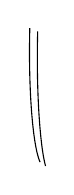
\begin{tikzpicture}
\draw (0,1.7) .. controls (-.02,.9) and (.04,.2) .. (.13,0);
\draw (.10,1.66) .. controls (.08,.9) and (.13,.2) .. (.20,-.05);
\end{tikzpicture}}}
Comme $\alpha$ se factorise
canoniquement en un hom surjectif
suivi d'un hom injectif de simplexes,
on est ramené à examiner séparément
les deux cas. Mais si $\alpha$ est surjectif
(``hom de dégénérescence''), \deleted{l'homomorphisme}
\inserted{on a $\alpha(0)=0$}
donc on est dans le cas déjà envisagé --
\deleted{\unsure{correspondant}}\inserted{d'ailleurs} dans ce cas
\diagram{\begin{tikzcd}[ampersand replacement=\&]
D^*_{\Delta_{r'}} \arrow[r] \& D^*_{\Delta_r}
\end{tikzcd}}
\unsure{se|a|à} décompose en des morphismes \unsure{:|;}
\diagram{(220)\qquad
\begin{tikzcd}[ampersand replacement=\&]
D^*_{d'_0,\unsure{\ldotp-\!-|-\!-},d'_{r'}}
\arrow[r] \&
D^*_{\unsure{d_0^{\deleted{\prime}}|d_0^*},-\!-,\unsure{d_r^{\deleted{\prime}}|d_r^*}}
\end{tikzcd},}
$(d_0,-\!-,d_r)$ est \unsure{déduite|déduit} de $(d'_0,-,d'_r)$
en \unsure{réécrivant} cette suite, en répétant certains
de ses éléments -- et \deleted{les} alors (220) est
un iso -- donc \uline{si $\alpha$ est un hom}
\margin{On voit que la considération des
$\widetilde{\Pi}_{d_0-d_r}$, $\Pi_{d_0,-d_r}$
pour $d_0,-\!-,d_r$ \unsure{non}
\unsure{\uline{strictement}|\uuline{strictement}}
décroiss. et celle de $\alpha^*$, pour $\alpha$
\unsure{non} \uline{stricts} croissants,
est de la poudre aux yeux, simplement !}
\margin{133}

\cotefile{147}
\scanpage{135}
\uline{de dégénérescence}, \uline{alors} (219) \uline{est un}\deleted{e}
\deleted{\unsure{équiv.}}\uline{isomorphisme}, de nature ess.\textsuperscript{t} triviale.

On est donc réduit à regarder le
cas d'une application \uline{injective} $\alpha$ (``opération
face''), et le \inserted{seul} cas qui \deleted{\unsure{pose}} pose problème
est bien sûr celui où $\alpha(0)\ne0$. Donc
\[
\tag{221}
\left\{\begin{aligned}
d_*&=\{d_0>d_1\cdots>d_r\},\quad\text{et si}\\
d'_*&=\{d'_0>d'_1>{-}>d'_{r'}\}\text{ est }
\text{\deleted{\unsure{une sous-suite}}}\inserted{\text{contenu dans }d_*},
\end{aligned}\right.
\]
$d'_0\ne d_0$ i.e. $d'_0<d_0$, il faut
\par\noindent définir l'hom
\diagram{\begin{tikzpicture}
\node (map) at (0,0) {\begin{tikzcd}[ampersand replacement=\&,column sep=2.8cm]
\Pi_1P^*_{d_0\deleted{\unsure{\geq}}d_1,\unsure{-\,-|\ldots},d_r}\arrow[r]\&
\Pi_1P^*_{d'_0,-,d'_r}
\end{tikzcd}};
\node[anchor=east] at (map.west) {$(222)$};
\node[anchor=south west,align=left,font=\footnotesize] at (1.1,0.75)
{attention, on a\\subrepticement changé\\de \unsure{notations|notation}, en interver-};
\node[anchor=north west,align=left,font=\footnotesize] at (1.1,-0.8)
{tissant $d_*$ et $d'_*$ !};
\draw (2.1,2.15) .. controls (1.1,1.95) and (0.6,1.35) .. (0.75,0.65)
;
\draw (2.1,0.65) .. controls (3.0,0.45) and (4.65,0.65) .. (5.0,0.45)
.. controls (5.25,0.15) and (5.25,-0.3) .. (5.1,-0.5)
.. controls (4.3,-0.55) and (2.95,-0.4) .. (2.1,-0.55);
\draw (1.65,-0.7) .. controls (0.65,-0.85) and (0.8,-1.4) .. (1.55,-1.5)
.. controls (2.6,-1.6) and (4.4,-1.25) .. (5.0,-1.2);
\end{tikzpicture}}
\margin{on se réduit au cas de $d_0,d_1,-,d_r$ strict.\textsuperscript{t} décroissants -- auquel \unsure{on} parvient aussitôt\unsure{. --|.} En fait, on est ramené au cas où $r'=r-1$, et où il s'agit de l'opération ``face de codim $1$'' pour laquelle $\alpha(0)\ne0$, donc correspondant :
\diagram{\begin{tikzcd}[ampersand replacement=\&]D_{d_0,d_1,-,d_r}\arrow[r]\&D_{d_1,-,d_r}\end{tikzcd}}}

Notons que l'on a
\diagram{$(223)\qquad$\begin{tikzcd}[ampersand replacement=\&]
D^{\unsure{\deleted{*}}}_{d_0,\unsure{-\,-|\ldots},d_r}\arrow[r]\&D_{d'_0,-,d'_{r'}}
\end{tikzcd}}
(mais \uline{non} un morphisme entre les
espaces avec $*$ !), qui est une immersion \inserted{locale}
d'\unsure{espaces|espace} \unsure{analytiques|analytique} \unsure{lisses|lisse}, de codim
$d_0-d'_0$, \deleted{qui}\inserted{\unsure{car il|ainsi|et}} s'insère dans le diagramme
\margin{134}

\cotefile{147}
\scanpage{136}
\mspage{67}
\diagram{$(22\deleted{\unsure{?}}4)\qquad$\begin{tikzcd}[ampersand replacement=\&]
D_{d_0,-,d_r}\arrow[r]\arrow[d]\&D_{d'_0\,--\,d'_{r'}}\arrow[d,no head,"{\unsure{}}" description]\\
D_{d_0,d'_0}\arrow[r]\&D_{d'_0}^{\deleted{\unsure{*}}}
\end{tikzcd}}
où les flèches verticales sont étales,
et la $2^{\mathrm{ième}}$ flèche horizontale est une
immersion loc.le de codim $\unsure{d_0|d^{\prime}_0}$\deleted{$\unsure{-}d'_0$. \unsure{On a|Quand}}
\[
\tag{225}\unsure{d|\delta}=d_0-d'_0
\]
[Dans le typique (auquel on se réduit)
où $\unsure{\{}d'_* = \{d_1\uline{>--} >d_r\}$, le diagramme
(224) est cartésien -- \deleted{\unsure{comme on voit|c'est à dire}}\inserted{plus \unsure{gén.\textsuperscript{t}|génér.\textsuperscript{t}}}, il
\unsure{reste} \deleted{\unsure{tjs|tjrs}} cartésien, \inserted{si $d'_0=d_1$} et c'est trivial.]
\margin{\uline{NB} Dans le cas général, on a
\diagram{\begin{tikzcd}[ampersand replacement=\&, column sep=small]
D_{d_*}\arrow[r,"{\text{fini étale}}"']\arrow[dd,dotted]\&D_{\unsure{\widetilde d'_*|\widetilde d_*}}\arrow[r]\arrow[d]\&D_{d'_*}\arrow[d]\\
\&D_{d_0,d'_0}\arrow[dl,dotted]\arrow[r,no head]\&D_{d'_0}\\
D_{d_0}\&\&
\arrow[ul,phantom,from=2-3,to=1-2,"{\text{cart}}" description]
\end{tikzcd}}}
Considérons le morphisme induit
\diagram{$(225)\qquad$\begin{tikzcd}[ampersand replacement=\&]D^*_{d_*}\arrow[r]\&D_{d'_*}\end{tikzcd}}
(Attention, on a mis un $*$ en exposant
à $D_{d_*}$ seulem\textsuperscript{t}, non : $D_{d'_*}$ !).

Nous munissons $D_{d'_*}$ du diviseur
$\Theta_{d'_*}$ image inverse de $\Theta_{d_0}$ sur $D_{d_0}$.
On désigne par $\Theta_{d'_*}^{(p)}$ le ``squelette
de dim $p$'' de $\Theta_{d'_*}^{p}$, et \deleted{\unsure{p}} on pose
\margin{135}

\cotefile{147}
\scanpage{137}

\[
(226)\qquad
\Theta_{d'_*}^{\unsure{d}*}\overset{\mathrm{def}}=
\Theta_{d'_*}^{\unsure{d}}\setminus
\Theta_{d'_*}^{\unsure{d+1|d1}}
\]
squelette ``privé'' de codim. $d$ de
$\Theta_{d'_*}$ dans $D_{d'_*}$.

Ceci posé, on sait que $225$ \unsure{\uline{induit}|\uuline{induit}}
un \deleted{morphisme} iso\uline{morphisme local}
\uline{de} $D_{d_*}$ \uline{sur}
\deleted{$\unsure{D_{d'_*}|\Theta_{d'_*}}$}
$\Theta_{d'_*}^{d*}$. Plus
précisément, \deleted{$\Theta_{d'_*}^{d*}$ s'identifie \unsure{à|\inserted{can.}} :}
\deleted{$\unsure{D_{(d_0,d'_0,-,d'_r)}}\ \unsure{:|.}\
D_{\widetilde d'_*}$, \unsure{où}}
\diagram{(22\unsure{7})\qquad
\begin{tikzcd}[ampersand replacement=\&]
\Theta_{d'_*}^{(d)} \&
D_{\widetilde d'_*}\arrow[l,"\sim"']
\end{tikzcd}}
où \deleted{$\unsure{d|d'}$}
\[
\widetilde d'_*=(d_0,d'_0,-\!-,d'_r)
\]
et cet isom. induit un isom
\diagram{(228)\qquad
\begin{tikzcd}[ampersand replacement=\&]
D_{\widetilde d'_*}^{*}\arrow[r,"\sim"]\&
\Theta_{d'_*}^{(d)*},
\end{tikzcd}}
d'autre part (223)
$D_{d_*}\mathrel{\text{---}}D_{d'_*}$ se
factorise en
\diagram{(229)\qquad
\begin{tikzcd}[ampersand replacement=\&]
D_{d_*}\arrow[r,no head]\&
D_{\widetilde d'_*}\arrow[r]
\arrow[d,phantom,"\rotatebox{90}{$\simeq$}" description]\&
D_{d'_*}\\
\&\Theta_{d'_*}^{(d)\unsure{*}}\&
\end{tikzcd}}
donc c'est un morphisme étale fini,
suivi \inserted{est} \unsure{d'un|\deleted{d'un}} morphisme d'inclusion de
$\Theta_{d'_*}^{(d)}$ dans $D_{d'_*}$. De plus, comme $D_{d_*}^{*}$ est
\margin{136}

\cotefile{148}
\scanpage{2}

\margin{(29.11.83)}

Soit $X$ surf. à bord compacte orientée, à
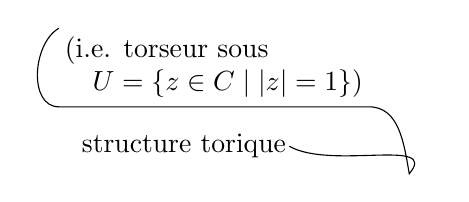
\begin{tikzpicture}[baseline=(torique.base)]
\node[anchor=west,inner sep=1pt] (torique) at (0,0) {structure torique};
\node[anchor=south west,inner sep=2pt,align=left] (torusnote) at (-.25,.5)
{\inserted{\begin{tabular}{@{}l@{}}(i.e. torseur sous\\
\quad$\mathbb U=\{z\in\mathbb C\mid |z|=1\}$)\end{tabular}}};
\draw (torusnote.north west) to[out=210,in=180] (torusnote.south west)
 -- (torusnote.south east) to[out=0,in=100] (4.2,-.35)
 to[out=50,in=-30] (torique.east);
\end{tikzpicture}
donnée sur les comp. connexes du bord.
On définit

\[
\begin{aligned}
\operatorname{SRT}(\unsure{X})={}&
\text{quotient du groupe des autom de }X
\text{ (\deleted{\unsure{en|on}} resp. l'orientation}\\
&\text{et les structures toriques) par la comp. neutre du}\\
&\text{sous-groupe }\operatorname{Aut}^!(\vec X)
\deleted{\unsure{\mathrm{bijec.}|\mathrm{diag}}}
\text{ \unsure{de|des} Aut qui induit}\\
&\text{l'identité sur }\partial X
\end{aligned}
\]

On a ainsi un dévissage de $\operatorname{SRT}(X)$ en trois étages

\[
\underbrace{S_{\unsure{*}}T^!(X)}_{
\operatorname{Aut}^!(\unsure{\vec X|\overline X})/
\text{comp. neutre}}
\qquad\mathbb U^I\qquad\unsure{\mathfrak S_I}
\qquad I=\pi_0(\partial X)
\]

ou encore

\[
\mathbb Z^I\qquad T(X)\qquad\mathbb U^I\qquad\unsure{\mathfrak S_I}
\]

En fait, on définit can! un sous-groupe
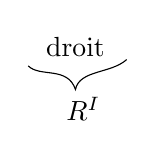
\begin{tikzpicture}[baseline=(ri.base)]
\node[inner sep=1pt] (ri) at (0,0) {$\mathbb R^I$};
\node[anchor=south] at (-.1,.55) {\inserted{droit}};
\draw (-.7,.55) .. controls (-.55,.4) and (-.2,.55) .. (-.1,.25)
 .. controls (-.05,.5) and (.35,.45) .. (.55,.63);
\end{tikzpicture}
de $\operatorname{SRT}(X)$
contenant $\mathbb Z^I$, de telle façon qu'on ait

\[
\underbrace{\operatorname{SRT}^!(X)}_{
\substack{\text{noyau de}\\
\operatorname{SRT}^!(\alpha)\to\unsure{\mathfrak S_I'|\mathfrak S_I^!}}}
=\mathbb R^I.S_*T^!(X)
\]

\diagram{
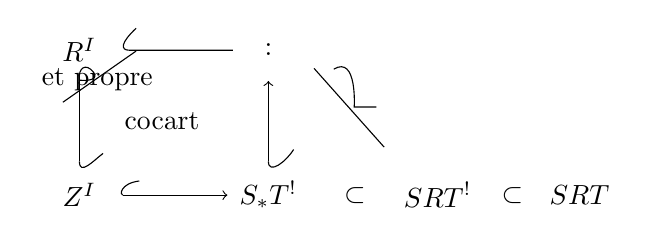
\begin{tikzpicture}[x=1cm,y=1cm]
\node (r) at (0,1.85) {$\mathbb R^I$};
\node (z) at (0,0) {$\mathbb Z^I$};
\node (p) at (2.4,1.85) {$\mathord{:}$};
\node (st) at (2.4,0) {$S_*T^!$};
\node at (3.5,0) {$\subset$};
\node at (4.55,0) {$\operatorname{SRT}^!$};
\node at (5.5,0) {$\subset$};
\node at (6.35,0) {$\operatorname{SRT}$};
\draw (.72,2.12) .. controls (.53,1.94) and (.51,1.84) .. (.64,1.84)
 -- (1.95,1.84);
% The upper end of this left stroke merges with cancelled lettering and a diagonal.
\draw (0,.43) -- (0,1.46);
\draw (0,1.46) .. controls (-.02,1.61) and (.08,1.69) .. (.18,1.56)
 .. controls (.24,1.47) and (.13,1.45) .. (0,1.46);
\draw (-.21,1.18) -- (.72,1.83);
\node[anchor=east] at (-.24,1.62) {$\unsure{\phantom{\uparrow}}$};
\draw (0,.43) .. controls (.0,.24) and (.18,.44) .. (.3,.53);
\node[anchor=west] at (.45,.94) {cocart};
\node[anchor=west] at (-.6,1.47) {\deleted{\unsure{et propre}}};
\draw[->] (.55,0) -- (1.88,0);
\draw (.76,.18) .. controls (.52,.15) and (.51,.0) .. (.55,0);
\draw[->] (2.4,.43) -- (2.4,1.45);
\draw (2.4,.43) .. controls (2.4,.25) and (2.63,.43) .. (2.72,.58);
% The following two source strokes have an unresolved reading (lambda / crossed 2).
\draw (2.98,1.61) -- (3.87,.61);
\draw (3.23,1.6) .. controls (3.53,1.78) and (3.49,1.12) .. (3.49,1.12)
 -- (3.77,1.12);
\node[anchor=west] at (3.91,1.12) {$\unsure{\phantom{\lambda}}$};
\end{tikzpicture}
}

i.e. on a

\margin{\uline{NB} $\operatorname{SUT}(X)\simeq
T(X)\times_{\unsure{\mathfrak S_I}}\operatorname{Aut}((T_i)_{i\in I})$}

\margin{Jusqu'ici on ne fait intervenir
que $S_*T^!(X)$, à l'exclusion de $S_*T(X)$,
dont la défini. exige une str. suppl.
$\uline{s}$, cf ci-dessous}

\diagram{
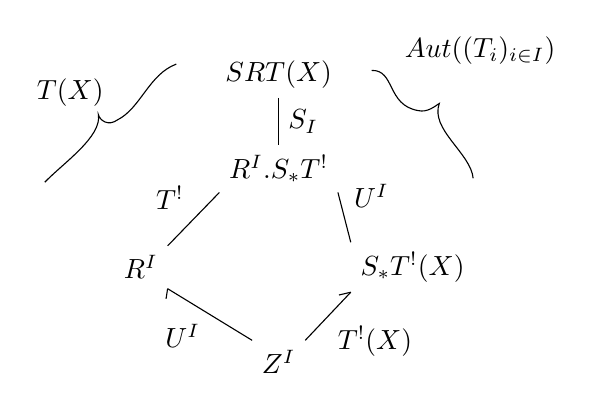
\begin{tikzpicture}[x=1cm,y=1cm]
\node (top) at (0,2.45) {$\operatorname{SRT}(X)$};
\node (mid) at (0,1.25) {$\mathbb R^I.\unsure{S_*T^!}$};
\node (left) at (-1.75,0) {$\mathbb R^I$};
\node (right) at (1.7,0) {$S_*T^!(X)$};
\node (bottom) at (0,-1.2) {$\mathbb Z^I$};
\draw (top.south) -- (mid.north) node[midway,right] {$\unsure{\mathfrak S_I}$};
\draw (mid.south west) -- (left.north east) node[midway,above left] {$T^!$};
\draw (mid.south east) -- (right.north west) node[midway,above right] {$\mathbb U^I$};
\draw (left.south east) -- (bottom.north west) node[midway,below left] {$\mathbb U^I$};
\draw (bottom.north east) -- (right.south west) node[midway,below right] {$T^!(X)$};
% Short terminal returns are drawn; their arrowhead status remains uncertain.
\draw (left.south east) -- ++(-.02,-.13);
\draw (right.south west) -- ++(-.15,-.035);
\node at (-1.24,-.4) {$\unsure{}$};
\node at (1.27,-.39) {$\unsure{}$};
\draw (-1.3,2.58) .. controls (-1.65,2.45) and (-1.75,2.02) .. (-2.05,1.87)
 .. controls (-2.16,1.79) and (-2.27,1.86) .. (-2.29,1.94)
 .. controls (-2.24,1.66) and (-2.74,1.32) .. (-2.97,1.08);
\node[anchor=east] at (-2.1,2.22) {$T(X)$};
\draw (1.18,2.5) .. controls (1.48,2.51) and (1.37,2.06) .. (1.77,1.99)
 .. controls (1.89,1.96) and (1.99,2.05) .. (2.04,2.08)
 .. controls (1.92,1.75) and (2.44,1.45) .. (2.47,1.13);
\node[anchor=south west] at (1.48,2.45) {$\operatorname{Aut}((T_i)_{i\in I})$};
\end{tikzpicture}
}

d'où
\diagram{
\begin{tikzpicture}[x=1cm,y=1cm]
\node (quot) at (0,0) {$\operatorname{SRT}\deleted{(X)}/\mathbb Z^I
 \overset{\text{déf}}=\operatorname{SUT}(X)$};
\node (prod) at (-.85,-1.1) {$T^!(X)\times\mathbb U^I$};
\draw[->] (-1.2,-.3) -- (-1.2,-.78);
\node at (1.42,-.62) {$\Big\}\ \unsure{\mathfrak S_I}$};
\draw (-3.0,-1.52) .. controls (-2.4,-1.6) and (-2.0,-1.54) .. (-1.62,-1.51)
 .. controls (-1.44,-1.71) and (-.92,-1.6) .. (-.4,-1.51)
 .. controls (.13,-1.64) and (.48,-1.64) .. (1.1,-1.45)
 .. controls (1.52,-1.41) and (1.85,-1.47) .. (2.0,-1.47);
\end{tikzpicture}
}

\[
(*)\qquad1\longrightarrow\mathbb U^I\longrightarrow
\operatorname{SUT}(X)\longrightarrow
\unsure{\deleted{\mathfrak S}T|T}(X)-1
\]

De plus, chaque fois qu'on se donne un
marquage, i.e. un pt \deleted{\unsure{de}}

\[
\uline{s}=(s_i)\in
\prod_{i\in I=\pi_0(\partial X)}
\deleted{\unsure{\mathbb U_i|(\mathbb U_i)|(T_i)}}T_i
\]

\margin{$T_i\unsure{=|:}$ comp. connexe (torique) de
$\partial X$ d'indice $i$\par\hspace{1.1cm}$\unsure{i|\varphi}$}

on trouve un plongement
\[
S_*T^{\deleted{\unsure{!}}}(X,\uline{s})\hookrightarrow\operatorname{SRT}(X)
\]
tel qu'on en \unsure{déduise|déduire}

\[
S_*T^{\deleted{\unsure{!}}}(X,\uline{s})
\mathbin{\wedge}_{\mathbb Z^I}\mathbb R^I
\simeq\operatorname{SRT}(X)
\]

\margin{1}

\cotefile{148}
\scanpage{3}

Une façon de le voir est de dire que
la donnée de $\uline{s}$ définit un scindage
\inserted{$\varphi_{\uline{s}}$} de
l'extension $(*)$ ci-dessus, \unsure{et que vu pour|et en tant que}
ss-groupe de $\operatorname{SRT}(X)$,
$S_1T(X,\uline{s})$ s'identifie
à l'image \unsure{inverse|\deleted{d'}inverse} de
\[
\varphi_{\uline{s}}(T(X))\subset\operatorname{SUT}(X)
\]
par l'hom. can
$\operatorname{SUR}(X)\mathrel{\unsure{\text{---}|\longrightarrow}}\operatorname{SUT}(X)$
de passage au quotient. Le chgt de
$\uline{s}$ en $\uline{s}'=u.\uline{s}$
transforme $\varphi_{\uline{s}}$ en
\[
\varphi_{\uline{s}'}=\operatorname{int}(u)\circ\varphi_{\uline{s}}
\]
donc (si $\widetilde u\in\mathbb R^I$ relève $u$\unsure{,|)} on trouve
\[
S_1T(X,\uline{s}')
=\operatorname{int}(\widetilde u)S_1T(X,\uline{s})\unsure{.|,}
\]

En termes de $\unsure{\overline X|\vec X}$, la définition de
$S_1T(X,\uline{s})$
dépend un choix $\uline{s}$ \uline{non-anodin},
par contre celle de $S_1RT(X)$ ne dépend que d'
un choix anodin, celui de la famille des
structures toriques $(t_i)_{i\in I}$.
De plus $\prod T_i$ comme
torseur sous $\unsure{\mathbb U^I|\mathbb M^I}$ se réalise
\inserted{(pas fidèlement d'ailleurs)}
comme \unsure{une classe|un des} de scindages de l'ext. $(*)$
(via autom. int. par $\mathbb U^I$)
$\bigl[$déduits de $\operatorname{SRT}(X)$
avec les structures suppl.$\unsure{\bigr\}|\bigr]}$
savoir\unsure{)|,} les inclusions

\diagram{
\begin{tikzpicture}[baseline=(current bounding box.center)]
\node (a) at (0,1.65) {$\mathbb{R}^{I}$};
\node (b) at (0,-1.65) {$S_1T^{!}(X)$};
\node (c) at (4.6,0) {$S\unsure{R|K}T(X)$};
\draw[->] (a.east) to[out=-35,in=165] (c.north west);
\draw (3.12,.73) .. controls (3.35,.66) and (3.52,.43) .. (3.73,.24);
\draw[->] (b.north east)--(c.south west);
\end{tikzpicture}
}

\unsure{coïncid.|coïncidant|coincident} sur $\mathbb Z^I$.

\margin{2}

\cotefile{148}
\scanpage{4}

Ceci dit, si on se donne un
multimarquage de $\partial X$, savoir pour
chaque $i\in I$ un $n_i\in\mathbb N^*$ et un
sous-\inserted{\unsure{$\mathbb Z_{n_i}$|$\mathbb Z/n_i$|$\mathbb Z n_i$}-}torseur
$T_i(n_i)\subset T_i$,
\deleted{\unsure{le groupe|les groupes|de groupe}} i.e
un $s_i\in T_i^{\wedge n_i}$, d'où
$\deleted{\unsure{\uline{s}\in}}$
\[
\uline{s}\in\prod_{i\in I}T_i^{\wedge n_i},
\]
alors le groupe de Teichmüller multimarqué
$S_{\unsure{*|1|g}}T(\unsure{X|\uline{X}},\uline{s})$,
généralisant le précédent, est
plongé dans $\operatorname{SRT}(X)$ de façon naturelle,
en prenant un $s_i^0$ dans chaque $T_i(n_i)$, d'où
$\uline{s}^0\in\prod T_i$ et
$ST(X,\uline{s}^0)\subset\operatorname{SRT}(X)$,
et on prend le ss-groupe
\[
ST(X,\uline{s})=ST(X,\uline{s}^0).
\prod_{i\in I}\frac1{n_i}\mathbb Z_i
\]
où $\mathbb Z_i$ est le $i$ème facteur de
$\mathbb Z^I\subset\operatorname{SRT}(X)$.

\margin{3}

\cotefile{148}
\scanpage{5}
\mspage{1}

\uline{Courbes} \inserted{exceptionnelles} \uline{de type} $(1,1)$ (sur $\mathbb C$)

A) \uline{Courbe} \inserted{ell.} \uline{anharmonique de type carré}

Cat. de ces courbes équivalente : celle des carrés
\unsure{combinatoires} orientés, i.e. des torseurs sous
\[
\mathbb Z/4\mathbb Z\simeq\mu_4(\mathbb C)\simeq
\begin{gathered}
\text{groupe des unités}\\
\text{algébriques \unsure{dans|de} }\mathbb Q[i]
\end{gathered}
\]
\margin{i.e. groupe des unités \unsure{dans|de} $\mathbb Z[i]$
(\unsure{anneau} des entiers de $\mathbb Q[i]$}

La donnée d'un tel torseur \inserted{($S$)} permet de tordre
$\mathbb E\ell_0\overset{\mathrm{def}}\simeq\mathbb C/\mathbb Z[i]$
et trouver
\[
\mathbb E\ell_0(S)\simeq\mathbb E\ell_0
\mathbin{\wedge}_{\mathbb Z/4\mathbb Z}S
\]

\margin{\figure{
% UPPER-DRAWING-BEGIN
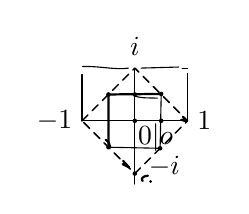
\begin{tikzpicture}[scale=.67,line cap=round,line join=round]
\draw[thin] (-1,0)--(-1,.88);
\draw[thin] (-.99,1.03)..controls(-.65,1.04)and(-.35,.96)..(-.12,1);
\draw[thin] (.12,1)--(.83,1.02);
\draw[thin] (.9,.99)--(1.0,.99);
\draw[thin] (1,.9)--(1,0);
\draw[dash pattern=on 3pt off 2.2pt,line width=.55pt] (-1,0)--(0,1)--(1,0)--(0,-1)--cycle;
\draw (-1,0)--(1,0);
\draw (0,-1.2)--(0,1);
\draw[thick] (-.5,-.5)--(-.5,.5)--(.5,.51);
\draw[thin] (.5,.48)--(.48,-.52)--(-.5,-.5);
\draw[thin] (0,.47)..controls(.15,.42)and(.32,.44)..(.43,.43);
\foreach \x/\y in {0/0,-.5/.5,0/.5,.5/.51,.5/0,.48/-.52,-.5/-.5,0/-1}
{\fill (\x,\y) circle (.043);}
\node[left] at (-1,0) {$-1$};
\node[right] at (1,0) {$1$};
\node[above] at (0,1.06) {$i$};
\node[right] at (.08,-.86) {$-i$};
\node[below right,inner sep=1pt] at (0,0) {$\unsure{0|o}$};
\draw[thick] (.25,-1.04)..controls(.12,-1.05)and(.12,-1.12)..(.15,-1.14);
\fill (.30,-1.15) circle (.028);

\draw[thick] (-.55,-.36)--(-.50,-.40)--(-.47,-.48);
\draw[thick] (.88,.02)--(.98,-.01)--(.91,.08);
\draw[thick] (-.22,-.76)--(-.11,-.88)--(-.23,-.82);
\end{tikzpicture}
% UPPER-DRAWING-END
}}

Si le carré est réalisé comme carré \inserted{euclidien}
dans un plan euclidien \inserted{$V_S$} (canoniquement), de centre
$\unsure{0|o}$,
\figure{
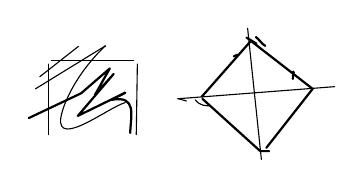
\begin{tikzpicture}[scale=.7,line cap=round,line join=round]
\begin{scope}[xshift=-1.45cm]
% CANCELED-DRAWING-BEGIN
% The cancellation strokes belong to the source drawing.
\draw (-1,-.7)--(-1,.58);
\draw (-.94,.65)--(.55,.65);
\draw (.62,.58)--(.6,-.7);
\draw[thin] (-1.15,.35)--(-.45,.9);
\draw[thin] (-1.23,.13)--(.04,.91);
\draw[thick] (-1.35,-.40)--(-.40,.05)--(.12,.50)--(-.15,.02)--(.19,.40)--(-.46,-.36)--(.40,.06);
\draw[thin] (.04,.91)..controls(-.35,.55)and(-.70,.0)..(-.77,-.40)
..controls(-.84,-.95)and(.12,-.19)..(.40,-.12);
\draw[thick] (.40,.06)--(.15,-.07)..controls(.62,.02)and(.50,-.35)..(.49,-.67);
% CANCELED-DRAWING-END
\end{scope}
\begin{scope}[xshift=1.35cm]
% LIVE-DRAWING-BEGIN
\draw[thick] (-1,0)--(-.12,1.0)--(1,.13)--(.16,-.94);
\draw[thick] (-1,-.05)--(.05,-1.0)--(.21,-1.0);
\draw (-1.45,-.05)--(1.4,.17);
\draw (.07,-1.15)--(-.18,1.23);
\draw[thick] (-.20,1.06)--(-.02,.95);
\draw[thick] (-.03,1.07)..controls(.03,1.03)and(.08,.94)..(.14,.91);
\draw[thick] (-.36,.75)--(-.43,.72);
\draw[thick] (.65,.44)--(.64,.31);
\draw[thin] (-1.13,-.07)..controls(-1.03,-.19)and(-.94,-.17)..(-.85,-.18);
\fill (-1,0) circle (.03);
\fill (.65,.43) circle (.03);
\draw[thin] (-1.43,-.05)--(-1.29,-.09);
% LIVE-DRAWING-END
\end{scope}
\end{tikzpicture}
}
on en déduit dans le plan (vectoriel via $\unsure{0|o}$) $V_S$
un syst. de deux \deleted{\unsure{axes} de}
coordonnées \inserted{mod. signes,}
via les diagonales, d'où un
\deleted{\unsure{lattice|entier}} \inserted{réseau}
\margin{\figure{
% LOWER-DRAWING-BEGIN
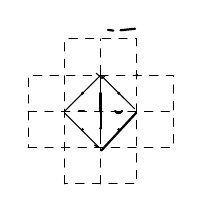
\begin{tikzpicture}[scale=.46,line cap=round,line join=round]
\draw[dashed] (-1,-2)--(-1,2)--(1,2)--(1,-2)--cycle;
\draw[dashed] (-2,-1)--(2,-1)--(2,1)--(-2,1)--cycle;
\draw[dashed] (-2,0)--(2,0);
\draw[dashed] (0,-2)--(0,-1.03);
\draw[dashed] (0,1.04)--(0,2);
\draw[thick] (.20,2.25)--(.35,2.23);
\draw[thick] (.55,2.24)--(.95,2.28);
\draw (-1,0)--(0,1)--(.94,.07);
\draw (-.99,-.05)--(-.04,-1);
\draw[thick] (.98,-.04)--(.02,-1.08);
\draw (0,-.89)--(0,1.14);
\draw[very thick] (0,0)--(0,.50);
\draw[thick] (0,-.47)--(0,0);
\draw[thin] (-.12,1.05)--(.04,.91)--(.12,.98);
\foreach \x/\y in {0/0,-.5/.5,.5/.5,-.5/-.5,.5/-.5,1/1,0/-.47}
{\fill (\x,\y) circle (.045);}

\draw[thick] (-.60,0)--(-.46,0);
\draw[thick] (.40,.01)..controls(.45,-.07)and(.52,-.07)..(.59,.01);
\draw[thin] (-.17,-.93)--(-.08,-.98)--(-.16,-1.00);
\end{tikzpicture}
% LOWER-DRAWING-END
}}
$\Gamma_S$ dans $V_S$ (sous-groupe discret de
rang $2$) et
\figure{
% ENCLOSURE-BEGIN
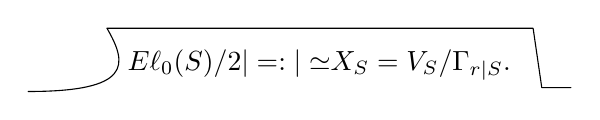
\begin{tikzpicture}[baseline=(F.base),line cap=round,line join=round]
\node[inner sep=3pt] (F) {$\mathbb E\ell_0(\unsure{S})\unsure{/2|=:|\simeq}X_S=V_S/\Gamma_{\unsure{r|S}}.$};
\draw ([xshift=-1.15cm,yshift=-.03cm]F.south west)
..controls([xshift=.16cm,yshift=-.03cm]F.south west)and([xshift=.12cm]F.west)..
([xshift=-.15cm,yshift=.16cm]F.north west)
--([xshift=.17cm,yshift=.16cm]F.north east)
--([xshift=.28cm,yshift=.02cm]F.south east)
--([xshift=.65cm,yshift=.02cm]F.south east);
\end{tikzpicture}
% ENCLOSURE-END
}

Il y a dans $X_S$ un élément d'ordre $2$ canonique
\inserted{$\eta_S$}
(stable par automorphismes), les deux autres él. d'
ordre $2$ sont échangés par le générateur $i$ de
$\mu_4(\mathbb C)\simeq\operatorname{Aut}(\unsure{X_S})$.
(\uline{NB} $\eta_S$ peut donc être défini

\margin{4}

\cotefile{148}
\scanpage{6}

\noindent
\begin{minipage}[t]{.46\textwidth}
\begin{center}
U N I V E R S I T E\\
DES SCIENCES ET TECHNIQUES\\
DU LANGUEDOC\\
\textasciicircum\textasciicircum\textasciicircum\textasciicircum\textasciicircum\textasciicircum\textasciicircum\textasciicircum\textasciicircum\textasciicircum\textasciicircum\textasciicircum\textasciicircum
\end{center}
\end{minipage}\hfill
\begin{minipage}[t]{.50\textwidth}
\vspace{.9\baselineskip}
Montpellier, le 14 octobre 1983
\end{minipage}

Service de la Scolarité

\begin{tabular}{@{}ll@{}}
Diffusion : & Liste A\\
MA/gs & N° 4375
\end{tabular}

\begin{center}
AVIS DE SOUTENANCE D'UNE THESE DE DOCTORAT DE 3e CYCLE

ECOLOGIE GENERALE ET APPLIQUEE OPTION ECOLOGIE AQUATIQUE

\texttt{========================================================}
\end{center}

\uline{NOM et Prénom du candidat} : MONTI Dominique

\uline{Titre de la thèse} : ``Recherches sur l'optimisation du plan d'échantillonnage employé pour la cartographie des peuplements benthiques. Application à la macrofaune benthique de l'étang de Pierre Blanche (Palavas, Hérault, France).

\uline{Date,-heure et lieu de soutenance prévus} : Le 2 novembre 1983 à 15 heures,\\
Salle de cours n° 9 - Université des Sciences et Techniques du Languedoc

\uline{Nom du Directeur de thèse} : M. AMANIEU

\uline{Désignation du Laboratoire où la thèse est préparée} : Laboratoire d'Hydrobiologie marine - U.S.T.L.

\uline{Analyse de l'ouvrage} : Cette réflexion porte sur le problème du choix du nombre et de l'organisation spatiale des points de prélèvement en écologie. Quel effort doit-on fournir pour un niveau de précision fixé ? Et où doit-on prélever ?

Ce travail est basé sur la réalisation de différents sous-échantillonnages d'une information initiale supposée maximale. Les différents sous-échantillonnages varient par le nombre et l'organisation spatiale des points de prélèvements ; et ils sont tous effectués à partir de la même liste d'objets.

Chaque sous-échantillonnage employé donnera naissance à une carte qui sera par la suite comparée à la carte dite ``de référence'' ; il restera à apprécier au vu de ces résultats si les cartes obtenues diffèrent de la référence, en quelles proportions et de quelle manière.

Les résultats théoriques sont appliqués à l'étude de la macrofaune benthique d'un étang littoral (l'étang de Pierre Blanche à Palavas, France).

\uline{Durée approximative des recherches ayant abouti à la thèse} : 3 ans

\uline{Composition du jury Proposé} : \begin{tabular}[t]{ll}
MM. & AMANIEU M.\\
& BLANC F.\\
& FRONTIER S.\\
& GRANDJOUAN G.\\
& LASSERRE G.
\end{tabular}

\begin{flushright}
P/ le Secrétaire Général,\\
L'Attachée Principale d'Administration\\
Scolaire et Universitaire,

\handwritten{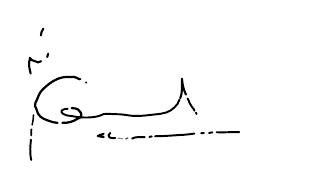
\begin{tikzpicture}[x=0.0013cm,y=-0.0013cm,line cap=round,line join=round]
\draw[line width=0.8pt] (812,700) .. controls (770,691) and (767,669) .. (719,678) .. controls (607,667) and (524,724) .. (445,800) .. controls (403,838) and (398,892) .. (375,927) .. controls (361,945) and (370,973) .. (384,995) .. controls (398,1060) and (437,1085) .. (499,1105) .. controls (538,1119) and (563,1127) .. (590,1127);
\draw[line width=0.8pt] (638,1127) .. controls (697,1130) and (749,1111) .. (780,1090) .. controls (824,1074) and (831,1051) .. (817,1026) .. controls (807,1002) and (787,984) .. (729,982);
\draw[line width=0.7pt] (690,989) .. controls (647,990) and (622,1005) .. (630,1024) .. controls (644,1046) and (686,1058) .. (719,1059) .. controls (758,1061) and (787,1076) .. (835,1074) .. controls (925,1077) and (972,1069) .. (1012,1054) .. controls (1047,1029) and (1093,1041) .. (1154,1042) .. controls (1219,1041) and (1262,1051) .. (1310,1057) .. controls (1403,1066) and (1479,1050) .. (1550,1044) .. controls (1629,1037) and (1690,1023) .. (1732,978) .. controls (1759,958) and (1776,930) .. (1784,900);
\draw[line width=0.75pt] (1792,886) .. controls (1812,837) and (1810,784) .. (1809,694) .. controls (1812,744) and (1824,803) .. (1848,850);
\draw[line width=0.7pt] (1864,888) .. controls (1882,920) and (1887,951) .. (1905,969) .. controls (1923,984) and (1928,1000) .. (1931,1008);
\draw[line width=0.7pt] (1946,1027) -- (1952,1040);
\draw[line width=0.55pt] (355,1050) .. controls (354,1079) and (350,1113) .. (342,1147);
\draw[line width=0.65pt] (334,1191) -- (332,1250);
\draw[line width=0.7pt] (330,1292) .. controls (325,1340) and (316,1414) .. (332,1490);
\draw[line width=0.75pt] (327,644) .. controls (319,607) and (308,570) .. (312,539) .. controls (315,516) and (319,500) .. (320,491) .. controls (324,514) and (346,514) .. (367,522) .. controls (390,535) and (413,544) .. (429,523);
\draw[line width=0.75pt] (427,271) .. controls (429,242) and (438,221) .. (452,205);
\draw[line width=0.75pt] (489,482) -- (499,450);
\fill (870,732) ellipse [x radius=10,y radius=12];
\draw[line width=0.75pt] (1042,1235) .. controls (1020,1242) and (993,1247) .. (984,1256) .. controls (1003,1257) and (1025,1266) .. (1043,1266);
\draw[line width=0.7pt] (1107,1226) .. controls (1087,1238) and (1082,1258) .. (1099,1270) .. controls (1115,1277) and (1141,1280) .. (1156,1275);
\draw[line width=0.45pt,opacity=0.45] (1183,1277) -- (1229,1282);
\draw[line width=0.55pt,opacity=0.65] (1259,1284) -- (1278,1276);
\draw[line width=0.7pt] (1321,1281) .. controls (1350,1263) and (1390,1266) .. (1444,1267);
\draw[line width=0.7pt] (1490,1265) -- (1513,1260);
\draw[line width=0.7pt] (1545,1258) .. controls (1660,1257) and (1735,1248) .. (1827,1244) .. controls (1871,1239) and (1901,1238) .. (1930,1232);
\draw[line width=0.7pt] (1997,1228) -- (2024,1226);
\draw[line width=0.7pt] (2074,1226) -- (2107,1220);
\draw[line width=0.7pt] (2149,1219) .. controls (2220,1224) and (2290,1214) .. (2370,1218);
\node[anchor=west] at (2430,850) {$\unsure{\phantom{A}}$};
\end{tikzpicture}}

A. GENTIL
\end{flushright}

\margin{5}

\cotefile{148}
\scanpage{7}
\mspage{2}

comme l'unique élément de \({}_2(X_S)\) qui
est fixe par $\operatorname{Aut}(X_S)\simeq\mathbb Z/4\mathbb Z$. En fait
\[
\inserted{(X_S)^{\unsure{f}i}\overset{\mathrm{def}}{=}\{x\in X_S\unsure{\deleted{\}}}\mid ix=x\}=\{e,\eta_S\}}
\]
\deleted{\unsure{$X$}} La surface top. $X_S$ a une déc. cell.
\inserted{\unsure{can|ces}} avec 1 sommet $e$, deux arêtes, une face,
\inserted{ces arêtes} correspondant aux deux mailles du réseau $\Gamma_S$.

On considère $X_S$ comme muni de cette décomposition.
Parfois c'est l'image inv. de celle-ci par $2\operatorname{id}_{X_S}$
qui est plus commode, 4 sommets (\unsure{formant|forment} \({}_2(X_S)\)),
\deleted{\unsure{quatre}} \inserted{huit} arêtes,
\deleted{(\uline{NB} \unsure{le}} \inserted{$4^{\unsure{\frown}}$} faces.
On peut considérer $\mathbb Z/4\mathbb Z\simeq\mu_4(\mathbb C)$
comme le groupe d'automorphismes commun de ces deux structures cellulaires.

\figure{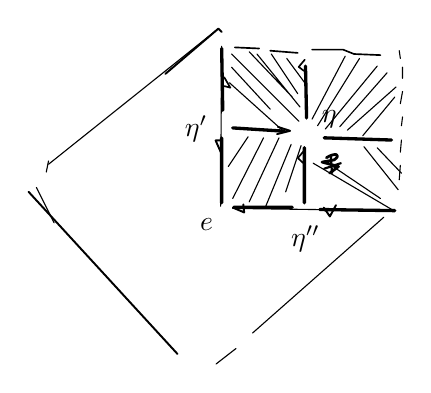
\begin{tikzpicture}[x=.014cm,y=-.014cm,line cap=round,line join=round]
% Detached oblique strokes surrounding the small square.
\draw[thin] (31,143)--(185,20);
\draw[line width=.7pt] (137,61)--(185,20)--(188,23);
\draw[thin] (31,140)--(29,150);
\draw[line width=.7pt] (13,168)--(148,315);
\draw[thin] (20,164)--(36,196);
\draw[thin] (183,324)--(201,310) (216,296)--(335,191);
% Interrupted upper and right edges; exposed left and lower edges.
\draw[thin] (188,36)--(187,181);
\draw[thin] (198,183)--(345,185);
\draw[line width=.6pt] (200,37)--(222,38) (232,40)--(257,42)
 (270,39)--(298,39)--(308,43)--(332,44);
\draw[thin] (349,40)--(350,47) (352,55)--(352,65)
 (352,77)--(350,88) (352,100)--(351,108)
 (351,121)--(350,132) (350,144)--(349,157);
% Heavy portions of the grid.
\draw[line width=1.2pt] (188,38)--(189,94) (188,119)--(188,178)
 (199,182)--(252,182) (277,184)--(345,185)
 (264,54)--(265,101) (263,128)--(263,178)
 (198,110)--(245,113) (281,119)--(342,121);
% Short angular projections on the thick grid strokes; direction remains unassigned.
\draw[line width=.7pt] (188,121.375)--(182.505,121.375)--(188,133.7);
\draw[line width=.6pt] (190.355,72.075)--(195.85,73.525)--(190.355,64.1);
\draw[line width=.7pt] (198.205,182.275)--(208.41,186.625)--(207.625,179.375);
\draw[line width=.7pt] (280.63,182.275)--(286.125,190.25)--(291.62,180.1);
\draw[line width=.7pt] (239.025,109.05)--(250.015,112.675)--(238.24,115.575);
\draw[line width=.6pt] (262.575,130.8)--(257.08,137.325)--(263.36,143.125);
\draw[line width=.6pt] (262.575,58.3)--(257.865,54.675)--(263.36,48.15);
% Hatching, preserving the changing directions.
\draw[thin] (195,69)--(244,113) (197,55)--(232,93)
 (197,43)--(258,104) (213,41)--(252,82)
 (220,43)--(259,91) (233,43)--(257,79) (247,47)--(264,70);
\draw[thin] (270,102)--(300,45) (275,108)--(313,47)
 (282,111)--(329,54) (295,109)--(338,60)
 (302,112)--(346,73) (316,117)--(345,82);
\draw[thin] (194,145)--(212,118) (198,174)--(226,119)
 (213,177)--(240,119) (228,181)--(251,125)
 (246,168)--(260,126);
\draw[thin] (271,142)--(344,185) (286,143)--(332,174)
 (317,127)--(348,166) (329,128)--(351,151);
% Overdrawn cluster below the central junction: no character identification.
\draw[line width=1pt] (283,137)..controls(291,132)and(297,134)..(290,139)
 --(279,141)--(294,145)--(286,151);
\draw[line width=.8pt] (287,135)--(288,151) (281,147)--(296,142);
\node[anchor=north east] at (189,183) {$e$};
\node[anchor=east] at (184,111) {$\eta'$};
\node[anchor=north] at (264,190) {$\eta''$};
\node[anchor=south west] at (270,119) {$\eta$};
\end{tikzpicture}}

Le deuxième est mieux \unsure{adaptée|adapté} pour la description du quotient
\[
\deleted{\unsure{X|X_S}\mathbb E\unsure{\ell|\ell_0}(\unsure{S|2})}\quad X_S/\pm1
\]
qui est une sphère, subdivisée en \deleted{deux} \inserted{faces} \unsure{carrées|carrés},
se raccordant suivant un équateur \deleted{carré}\unsure{,|.}
subdivisé en quatre arêtes par $e^{\unsure{\natural|q}},\eta^{\unsure{\natural|q}},\eta'^{\unsure{\natural|q}},\eta''^{\unsure{\natural|q}}$.

\figure{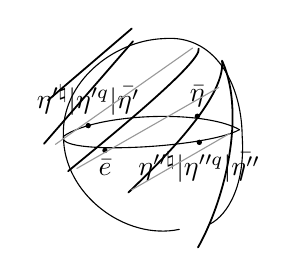
\begin{tikzpicture}[scale=.85,line cap=round,line join=round]
% The outline is interrupted near its lower-right end.
\draw (.45,-1.42)..controls(-.35,-1.59)and(-1.28,-.9)..(-1.28,-.03)
 ..controls(-1.32,.77)and(-.54,1.4)..(.21,1.43)
 ..controls(.98,1.5)and(1.38,.76)..(1.39,-.02)
 ..controls(1.44,-.75)and(1.18,-1.2)..(.91,-1.34);
\draw (-1.28,-.03)..controls(-.8,.31)and(.8,.38)..(1.35,.07);
\draw (-1.28,-.03)..controls(-1.42,-.32)and(.85,-.21)..(1.35,.07);
\fill (-.91,.13) circle (.04);
\fill (.72,.27) circle (.04);
\fill (-.66,-.24) circle (.04);
\fill (.75,-.12) circle (.04);
\node[above] at (-.91,.13) {$\unsure{\eta'^{\natural}|\eta'^{q}|\bar{\eta'}}$};
\node[above] at (.72,.27) {$\unsure{\bar\eta}$};
\node[below] at (-.66,-.24) {$\bar e$};
\node[below] at (.75,-.12) {$\unsure{\eta''^{\natural}|\eta''^{q}|\bar{\eta''}}$};
% Cancellation strokes through the whole drawing.
\draw[line width=.65pt] (-1.51,.51)--(-.26,1.58)
 (-1.57,-.14)--(-.24,1.39)
 (-1.21,-.55)..controls(-.49,.04)and(.79,1.09)..(.74,1.28)
 (-.31,-.87)..controls(.05,-.52)and(1.15,.51)..(1.09,1.1)
 (1.09,1.1)..controls(1.45,.3)and(1.13,-.98)..(.73,-1.69);
\draw[thin,black!40] (-1.4,-.15)--(.65,1.29)
 (-1.08,-.51)--(1.04,.7) (-.26,-.83)--(1.2,.01);
\end{tikzpicture}}

\figure{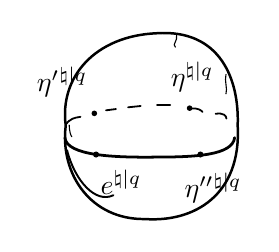
\begin{tikzpicture}[x=.55cm,y=.55cm,line cap=round,line join=round]
\draw[line width=.9pt] (-1.96,.08) .. controls (-2.11,1.20) and (-1.28,2.15) .. (.14,2.21) .. controls (1.61,2.31) and (2.05,1.14) .. (2.01,.08) .. controls (2.10,-1.53) and (1.00,-2.16) .. (-.13,-2.08) .. controls (-1.37,-2.10) and (-2.10,-1.05) .. (-1.96,.08);
\draw[line width=1.0pt] (-1.98,-.20) .. controls (-1.94,-.62) and (-.83,-.66) .. (.09,-.65) .. controls (1.04,-.65) and (1.89,-.61) .. (1.94,-.20);
\draw[line width=.65pt] (-1.96,.10) .. controls (-1.86,.24) and (-1.76,.26) .. (-1.62,.28);
\draw[line width=.65pt] (-1.03,.43)--(-.80,.46);
\draw[line width=.65pt] (-.52,.50)--(-.23,.53);
\draw[line width=.65pt] (.15,.55)--(.45,.55);
\draw[line width=.65pt] (.94,.47) .. controls (1.09,.49) and (1.17,.43) .. (1.20,.39);
\draw[line width=.65pt] (1.50,.35) .. controls (1.69,.38) and (1.75,.30) .. (1.75,.24);
\fill (-1.30,.36) circle (.065);
\fill (.90,.48) circle (.065);
\fill (-1.26,-.59) circle (.070);
\fill (1.15,-.59) circle (.070);
\draw[line width=.7pt] (-1.93,-.49) .. controls (-1.75,-1.20) and (-1.27,-1.73) .. (-.86,-1.53);
\draw[line width=.4pt] (.60,2.18) .. controls (.63,2.02) and (.49,1.96) .. (.57,1.89);
\draw[line width=.4pt] (1.74,1.26) .. controls (1.70,1.10) and (1.78,.94) .. (1.74,.81);
\draw[line width=.4pt] (-1.88,.09) .. controls (-1.88,-.05) and (-1.84,-.16) .. (-1.82,-.18);
\node[above left] at (-1.24,.51) {$\eta'{}^{\unsure{\natural|q}}$};
\node[above] at (.96,.63) {$\eta^{\unsure{\natural|q}}$};
\node[below right] at (-1.38,-.72) {$e^{\unsure{\natural|q}}$};
\node[below] at (1.44,-.78) {$\eta''{}^{\unsure{\natural|q}}$};
\end{tikzpicture}}

\margin{6}

\cotefile{148}
\scanpage{8}

\begin{minipage}[c]{.43\linewidth}\centering
U N I V E R S I T E\\
DES SCIENCES ET TECHNIQUES\\
\begin{tabular}{@{}l@{}}
\texttt{DU LANGUEDOC}\\[-.6ex]
\texttt{-{}-{}-{}-{}-{}-{}-{}-{}-{}-{}-{}-}
\end{tabular}

Service de la Scolarité\\
MA/GJ\\
Diffusion : Liste A\\
N° : 4679
\end{minipage}\hfill
\begin{minipage}[c]{.54\linewidth}\raggedleft
Montpellier, le 20 octobre 1983
\end{minipage}


\begin{center}
\begin{tabular}{@{}l@{}}
\texttt{AVIS DE SOUTENANCE D'UNE THESE DE DOCTEUR INGENIEUR}\\[-.6ex]
\texttt{-{}-{}-{}-{}-{}-{}-{}-{}-{}-{}-{}-{}-{}-{}-{}-{}-{}-{}-{}-{}-{}-{}-{}-{}-{}-{}-{}-{}-{}-{}-{}-{}-{}-{}-{}-{}-{}-{}-{}-{}-{}-{}-{}-{}-{}-{}-{}-{}-{}-{}-{}-}
\end{tabular}

\begin{tabular}{@{}l@{}}
\texttt{AUTOMATIQUE}\\[-.6ex]
\texttt{-{}-{}-{}-{}-{}-{}-{}-{}-{}-{}-}
\end{tabular}
\end{center}

\uline{Nom et prénom du candidat} : SITOHANG Benhard

\uline{Titre de la thèse} : LINAIRE : SYSTEME DE GESTION DE BASES DE DONNEES RELATIONNELLES SUR MICRO-ORDINATEUR.

\uline{Date, heure et lieu de soutenance prévus:} 28 OCTOBRE 1983 à 14h30 - CRIG USTL

\uline{Nom du Directeur de thèse} : Monsieur le Professeur B. FILLIATRE

\uline{Désignation du laboratoire où la thèse est préparée} : CRIG USTL

\uline{Résumé de la thèse} :

La conception et la réalisation d'un Système de Gestion de Bases de Données Relationnelles sur micro-ordinateur, que nous avons baptisé ``LINAIRE'', est le sujet de cette thèse.

Nous mettons l'accent sur trois points principaux :

1. BOUCLE MULTI-NIVEAUX ; c'est une technique du traitement de données, permettant d'éviter l'utilisation des relations intermédiaires comme résultats des opérateurs relationnels, ce qui serait particulièrement pénalisant pour un micro-ordinateur possédant une mémoire centrale limitée.

2. STRUCTURE INTERNE DE LA BASE ; elle est multiple, afin de préserver au mieux les performances tout en offrant en particulier la possibilité d'accélérer le traitement de l'opérateur relationnel ``équi-joint''.

3. L'adaptation sur un micro-ordinateur du langage de manipulation de QUERY-BY-EXAMPLE (langage de haut niveau, interactif, et tabulaire).

\uline{Durée approximative des recherches ayant abouti à la thèse} : 2 ans

\uline{Composition du jury proposé} :

\begin{tabular}{ll}
MM. & FILLIATRE B.\\
& CHEIN M.\\
& PICHAT E.\\
& PIROTTE A.\\
& PRUNET F.
\end{tabular}

\begin{center}
P. le Secrétaire Général,\\
l'Attachée Principale d'Administration Scolaire\\
et Universitaire,

\figure{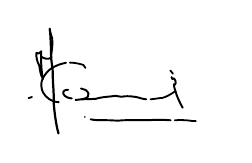
\begin{tikzpicture}[x=0.0011cm,y=-0.0011cm,line cap=round,line join=round]
\draw[line width=0.8pt] (630,126) .. controls (639,180) and (639,223) .. (642,282) .. controls (647,355) and (644,413) .. (649,481) .. controls (653,537) and (666,578) .. (666,648) .. controls (665,762) and (681,856) .. (676,973) .. controls (683,1080) and (704,1243) .. (732,1336);
\draw[line width=0.65pt] (637,170) .. controls (678,249) and (660,350) .. (646,436);
\draw[line width=0.7pt] (533,386) .. controls (521,416) and (491,416) .. (477,405) .. controls (471,455) and (488,516) .. (509,548) .. controls (517,592) and (523,665) .. (552,706) .. controls (536,630) and (532,544) .. (530,463) .. controls (528,431) and (535,412) .. (533,386);
\draw[line width=0.7pt] (532,448) .. controls (568,472) and (604,483) .. (645,463);
\draw[line width=0.65pt] (1043,579) .. controls (1038,551) and (1011,530) .. (976,532) .. controls (941,527) and (902,513) .. (863,517);
\draw[line width=0.7pt] (818,520) .. controls (755,530) and (710,549) .. (655,580) .. controls (610,608) and (572,658) .. (550,699) .. controls (521,754) and (533,826) .. (555,865) .. controls (590,925) and (649,969) .. (735,975);
\draw[line width=0.7pt] (844,831) .. controls (799,832) and (778,847) .. (789,880) .. controls (804,912) and (846,929) .. (886,931);
\draw[line width=0.7pt] (992,816) .. controls (1030,823) and (1066,836) .. (1079,875) .. controls (1090,907) and (1064,926) .. (1020,937) .. controls (981,946) and (951,945) .. (929,949) .. controls (1006,938) and (1085,941) .. (1162,936) .. controls (1213,919) and (1276,914) .. (1346,907) .. controls (1383,896) and (1400,903) .. (1433,908) .. controls (1453,915) and (1476,913) .. (1493,907) .. controls (1542,903) and (1578,908) .. (1625,914) .. controls (1680,925) and (1697,938) .. (1747,941);
\draw[line width=0.65pt] (1797,941) .. controls (1849,938) and (1885,927) .. (1935,925) .. controls (1985,911) and (2032,882) .. (2081,849);
\draw[line width=0.65pt] (2025,608) -- (2055,645);
\draw[line width=0.7pt] (2039,685) .. controls (2044,706) and (2047,716) .. (2068,700) .. controls (2082,712) and (2090,735) .. (2087,755) .. controls (2084,772) and (2071,779) .. (2067,768) .. controls (2057,792) and (2081,811) .. (2084,845) .. controls (2097,898) and (2130,973) .. (2168,1039);
\draw[line width=0.65pt] (386,928) -- (425,915);
\fill (1037,1145) ellipse [x radius=10,y radius=12];
\draw[line width=0.7pt] (1104,1173) .. controls (1154,1185) and (1207,1182) .. (1274,1183) .. controls (1339,1181) and (1411,1194) .. (1475,1184) .. controls (1576,1180) and (1668,1184) .. (1768,1183) .. controls (1851,1177) and (1939,1177) .. (2029,1184);
\draw[line width=0.65pt] (2077,1184) .. controls (2135,1179) and (2189,1181) .. (2248,1188) .. controls (2275,1192) and (2298,1196) .. (2320,1193);
\node[anchor=west] at (2420,900) {\unsure{}};
\end{tikzpicture}}

A. GENTIL
\end{center}

\margin{7}

\cotefile{148}
\scanpage{9}
\mspage{3}

B) Courbes \inserted{ell.} anharmoniques de type hexagonal.

La catégorie de ces courbes équivalente : celle des hexagones orientés,
i.e. des torseurs $S$ sous
\[
\begin{aligned}
\mathbb Z/6\mathbb Z&\simeq\mu_6(\mathbb C)\simeq
\text{groupe des}\\
&\qquad\qquad\text{unités \inserted{\unsure{alg.}} de }Q\left(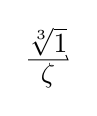
\begin{tikzpicture}[baseline=(rad.base)]
\node[inner sep=0pt] (rad) {$\sqrt[3]{1}$};
\draw[line width=.35pt] ([yshift=-1pt]rad.south west) -- ([yshift=-1pt]rad.south east) -- ++(-.025,.06);
\node[below=2pt,inner sep=0pt] at (rad.south) {$\zeta$};
\end{tikzpicture}\right)\\
&\simeq\text{groupe des unités \unsure{\begin{tikzpicture}[x=.04em,y=-.04em,line cap=round,line join=round,baseline=-.15ex]
\draw[line width=.35pt] (0,14) .. controls (5,14) and (13,8) .. (11,3)
 .. controls (10,0) and (7,0) .. (6,3)
 .. controls (3,8) and (8,12) .. (23,14);
\end{tikzpicture}}}\\
&\qquad\text{\uline{\unsure{\deleted{de}}}}\quad \deleted{\mathbb Z[\zeta]\unsure{=}\mathbb Z[T]/}\\
&\qquad \mathbb Z[\zeta]=\mathbb Z[T]/(1+T+T^2)\\
&\qquad (\zeta=\exp 2i\pi/\unsure{3})
\end{aligned}
\]

\figure{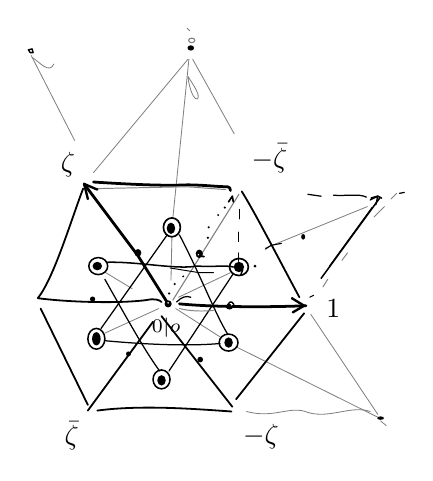
\begin{tikzpicture}[x=.012cm,y=-.012cm,line cap=round,line join=round]
% Exposed pale construction strokes and their interrupted ends.
\draw[gray,line width=.3pt] (172,921) -- (218,1011);
\draw[gray,line width=.3pt] (173,923) .. controls (181,928) and (191,941) .. (196,930);
\draw[gray,line width=.3pt] (238,1045) -- (338,925);
\draw[gray,line width=.3pt] (343,925) -- (387,1004);
\draw[gray,line width=.3pt] (339,925) -- (322,1093);
\draw[gray,line width=.3pt] (338,943) .. controls (342,950) and (352,963) .. (348,967)
  .. controls (342,968) and (338,947) .. (338,943);
\draw[gray,line width=.3pt] (321,1114) -- (320,1159);
\draw[gray,line width=.3pt] (251,1151) -- (279,1168);
\draw[gray,line width=.3pt] (325,1189) -- (372,1219);
\draw[gray,line width=.3pt] (390,1230) -- (539,1304);
\draw[gray,line width=.3pt] (250,1215) -- (307,1189);
\draw[gray,line width=.3pt] (328,1177) -- (383,1151);
\draw[gray,line width=.3pt] (468,1195) -- (539,1301);
\draw[gray,line width=.3pt] (400,1298) .. controls (430,1306) and (446,1291) .. (465,1299)
  .. controls (488,1306) and (511,1291) .. (531,1298);
\draw[gray,line width=.3pt] (420,1125) -- (528,1081);
% Outer sides: retain the gaps at the exposed junctions.
\draw[line width=.65pt] (227,1062) .. controls (215,1093) and (196,1157) .. (179,1178)
  .. controls (209,1182) and (263,1184) .. (294,1180)
  .. controls (303,1178) and (308,1180) .. (310,1182);
\draw[line width=.65pt] (182,1189) -- (232,1291);
\draw[line width=.65pt] (242,1297) .. controls (288,1291) and (342,1295) .. (384,1298);
\draw[line width=.65pt] (389,1285) -- (461,1194);
\draw[line width=.65pt] (395,1065) .. controls (410,1089) and (437,1142) .. (456,1177);
\draw[line width=.65pt] (310,1197) -- (385,1293);
\draw[line width=.65pt] (232,1297) -- (301,1203);
\draw[gray,line width=.4pt] (322,1180) -- (392,1068);
% Heavy top edge and its visible downward terminal curl.
\draw[line width=1pt] (238,1055) .. controls (285,1058) and (315,1059) .. (337,1058)
  .. controls (354,1058) and (369,1060) .. (380,1060)
  .. controls (382,1060) and (383,1062) .. (383,1064);
\draw[gray,line width=.35pt] (240,1062) -- (337,1060) -- (378,1063);
\node[above,inner sep=0pt,font=\scriptsize] at (382,1054) {\unsure{}};
% Two exposed directed heavy radii, drawn with their visible wings.
\draw[line width=1pt] (317,1184) -- (285,1133) -- (228,1057);
\draw[line width=.85pt] (232,1073) -- (228,1057) -- (242,1063);
\draw[line width=1pt] (329,1184) .. controls (359,1187) and (413,1188) .. (463,1186);
\draw[line width=.85pt] (448,1178) -- (461,1186) -- (449,1193);
% Inner triangular strokes, retaining their irregular paths.
\draw[line width=.45pt] (316,1111) -- (246,1210);
\draw[line width=.45pt] (329,1111) .. controls (351,1153) and (367,1195) .. (380,1216);
\draw[line width=.45pt] (250,1223) .. controls (292,1227) and (338,1229) .. (372,1226);
\draw[line width=.45pt] (250,1158) .. controls (272,1197) and (293,1235) .. (308,1255);
\draw[line width=.45pt] (318,1255) -- (386,1152);
\draw[line width=.55pt] (252,1140) .. controls (285,1139) and (326,1148) .. (347,1144)
  .. controls (365,1145) and (380,1143) .. (386,1145);
\draw[line width=.35pt] (319,1146) -- (350,1151) -- (365,1151);
% Individually visible marks on the dotted oblique and vertical strokes.
\foreach \x/\y/\r in {318/1173/1.3,324/1163/1.3,333/1155/1.1,359/1114/1.3,360/1103/1.2,370/1090/1.1,377/1082/1.3}{\fill (\x,\y) circle[radius=\r];}
\draw[line width=.6pt] (381,1076) -- (385,1070) -- (386,1076);
\draw[line width=.35pt] (393,1084) -- (393,1094) (392,1108) -- (392,1118) (391,1130) -- (391,1139);
% Exposed right-hand extension, parallel strokes, and short marks.
\draw[line width=.45pt] (465,1068) -- (479,1070);
\draw[line width=.45pt] (492,1069) .. controls (506,1070) and (519,1067) .. (527,1071);
\draw[line width=.6pt] (532,1072) -- (539,1070) -- (543,1072);
\draw[line width=.55pt] (479,1157) -- (541,1072);
\draw[line width=.45pt] (488,1144) -- (533,1082);
\draw[gray,line width=.35pt] (481,1166) -- (486,1158) (501,1138) -- (507,1130) (535,1092) -- (546,1081) (553,1073) -- (559,1067);
\draw[line width=.45pt] (562,1067) -- (567,1066);
\draw[line width=.4pt] (420,1126) -- (426,1122) -- (437,1120);
\draw[line width=.4pt] (467,1177) -- (471,1175);
% Six irregular ringed points with dark centers.
\draw[line width=.6pt] (321,1103) ellipse[x radius=9,y radius=10];
\fill (320,1104) ellipse[x radius=4.5,y radius=6];
\draw[line width=.6pt] (392,1145) ellipse[x radius=10,y radius=9];
\fill (392,1145) circle[radius=5.5];
\draw[line width=.55pt] (381,1225) ellipse[x radius=10,y radius=9];
\fill (381,1225) ellipse[x radius=4.5,y radius=5.5];
\draw[line width=.55pt] (310,1264) ellipse[x radius=9,y radius=10];
\fill (310,1265) ellipse[x radius=4.5,y radius=5.5];
\draw[line width=.55pt] (241,1221) ellipse[x radius=9,y radius=11];
\fill (241,1221) ellipse[x radius=4.5,y radius=7];
\draw[line width=.55pt] (243,1144) ellipse[x radius=10,y radius=9];
\fill (242,1144) ellipse[x radius=5,y radius=4.5];
% Filled marks and the three exterior marked points.
\fill (237,1179) circle[radius=2.8];
\fill (285,1130) ellipse[x radius=3.6,y radius=4];
\fill (350,1131) ellipse[x radius=3.8,y radius=4.5];
\draw[line width=.65pt] (350,1133) -- (355,1134);
\fill (382,1187) ellipse[x radius=3.8,y radius=3];
\draw[line width=.5pt] (380,1185) .. controls (383,1179) and (387,1183) .. (387,1187);
\fill (275,1237) circle[radius=2.6];
\fill (351,1243) circle[radius=3];
\fill (460,1113) ellipse[x radius=2.1,y radius=3];
\fill (409,1144) circle[radius=1.6];
\fill (317,1184) circle[radius=3.8];
\draw[line width=.5pt] (169,915) -- (173,914) -- (174,918) -- (171,918) -- cycle;
\draw[gray,line width=.4pt] (342,905) ellipse[x radius=3.3,y radius=2.4];
\fill (341,913) ellipse[x radius=3.5,y radius=2.8];
\draw[gray,line width=.3pt] (337,892) -- (340,895);
\fill (542,1305) ellipse[x radius=3.6,y radius=1.8];
\draw[gray,line width=.3pt] (542,1308) -- (548,1313);
% Further exposed returns and white apertures checked in the blind audit.
\draw[line width=.45pt] (326,1182) .. controls (331,1177) and (336,1175) .. (341,1177);
\draw[gray,line width=.35pt] (329,1189) .. controls (341,1192) and (354,1192) .. (365,1191);
\draw[line width=.5pt] (531,1074) -- (539,1070) -- (537,1079);
\draw[line width=.55pt] (388,1143) -- (396,1148) -- (394,1153);
\fill[white] (317,1183) circle[radius=1.0];
\fill[white] (349,1132) circle[radius=.8];
\fill[white] (384,1185) circle[radius=.9];
% Written labels; the small central round label remains ambiguous.
\node[anchor=east,inner sep=1pt] at (222,1037) {$\zeta$};
\node[anchor=west,inner sep=1pt] at (402,1030) {$-\bar\zeta$};
\node[anchor=west,inner sep=1pt] at (481,1189) {$1$};
\node[anchor=east,inner sep=1pt] at (226,1324) {$\bar\zeta$};
\node[anchor=west,inner sep=1pt] at (393,1325) {$-\zeta$};
\node[inner sep=0pt,font=\scriptsize] at (315,1209) {$\unsure{0|o}$};
\node[inner sep=0pt,font=\scriptsize] at (478,1261) {\unsure{}};
\end{tikzpicture}}

\deleted{\unsure{On pourra|On pose}} \inserted{On pose}
\[
\mathbb E\ell_1\deleted{(\unsure{S})}\simeq\mathbb C/\mathbb Z[\zeta]
\]
\[
\mathbb E\ell_1(S)\simeq\mathbb E\ell_1\mathbin{\wedge}_{\mathbb Z/6\mathbb Z}S
\]

\uline{Construction} On réalise l'hexagone \unsure{comb.|orient.} $S$ \unsure{euclidiennem\textsuperscript{t}|euclidiennement} (canonique), dans \unsure{vectoriel} euclidien $V_S$, \deleted{\unsure{centre|avec}} \inserted{origine} \unsure{étant|\inserted{étant}} le barycentre de $S$. On désigne par $V_S$ le \deleted{\unsure{lattice}} \inserted{réseau} engendré par $S$, et
\[
X_S\unsure{=|\simeq}\mathbb E\ell_1(S)\simeq V_S/\Gamma_S
\]
La structure euclidienne \uline{orientée} de $V_S$ définit la structure complexe de $X_S$.

\margin{8}

\cotefile{148}
\scanpage{10}

\noindent\begin{minipage}[t]{0.43\textwidth}
\centering
U N I V E R S I T E\\
DES SCIENCES ET TECHNIQUES\\
DU LANGUEDOC\\
\textasciicircum\textasciicircum\textasciicircum\textasciicircum\textasciicircum\textasciicircum\textasciicircum\textasciicircum\textasciicircum\textasciicircum\textasciicircum\textasciicircum\textasciicircum
\end{minipage}\hfill
\begin{minipage}[t]{0.49\textwidth}
\raggedleft
\vspace{1.5\baselineskip}
Montpellier, le 18 octobre 1983
\end{minipage}

Service de la Scolarité

Diffusion : Liste A\\
AM/gs \qquad N° 4570

\begin{center}
AVIS DE SOUTENANCE D'UNE THESE DE DOCTEUR-INGENIEUR

``ECOLOGIE GENERALE ET APPLIQUEE \quad option \quad ECOLOGIE TERRESTRE''

\texttt{============================================================}
\end{center}

\uline{NOM et prénom du candidat} : MOUFADDAL Mohamed

\uline{Titre de la thèse} : ``CONTRIBUTION A L'ETUDE DES POSSIBILITES D'EXTENSION\\
DU CEDRE DE L'ATLAS EN DEHORS DE SON AIRE ACTUELLE''

\uline{Date, heure et lieu de soutenance p\unsure{\deleted{\illegible{1}}}révus} : Le 28 octobre 1983 à 14 heures\\
à l'Institut de Botanique

\uline{Nom du directeur de thèse} : M. GODRON Michel

\uline{Désignation du laboratoire où la thèse est préparée} : Centre d'Etudes\\
Phytosociologiques et écologiques Louis Emberger (CNRS)

\uline{Aanlyse de l'ouvrage} : L'objet de cette étude étant de cerner les\\
possibilités d'extension du Cèdre (\uline{Cedrus atl\unsure{\deleted{\illegible{1}}}a}n\uline{tica} Manetti) en dehors de\\
son aire actuelle, il a fallu, après une analyse de l'histoire de répartition du\\
Cèdre, préciser les facteurs climatiques responsables de la distribution\\
actuelle.

Les régions où l'introduction du Cèdre est possible,\\
sont déterminées à partir de l'étude climatique de stations situées à l'intérieur\\
et à l'extérieur de l'aire du Cèdre, et par une étude écologique et dendromé-\\
trique comparative de quelques plantations.

\uline{Durée approximative des recherches ayant abouti à la thèse} : 5 ans

\uline{Composition du jury proposé} : \begin{tabular}[t]{ll}
MM. & GODRON M.\\
& BEDEL J.\\
& SCHOENENBERGER A.\\
& ROMANE F.\\
& DAGET Ph.
\end{tabular}

\begin{flushright}
P/ le Secrétaire Général,\\
l'Attachée principale d'administration\\
scolaire et universitaire,

% Signature: the alphabetic proposal A. Gentil remains undecided.
\unsure{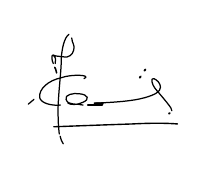
\begin{tikzpicture}[x=0.012cm,y=-0.012cm,line cap=round,line join=round,baseline=-0.4ex]
\draw[line width=0.45pt] (57,12) .. controls (52,16) and (50,26) .. (49,36)
  .. controls (49,52) and (46,71) .. (45.5,91)
  .. controls (45.5,109) and (46.5,114) .. (46.8,117.7);
\draw[line width=0.45pt] (47.7,120) .. controls (48.2,123) and (49.6,126) .. (51,128);
\draw[line width=0.45pt] (60,16) .. controls (60,21) and (64,24) .. (62,29)
  .. controls (61,34) and (56,37) .. (52,36)
  -- (43,35) .. controls (41,33.8) and (39,33.5) .. (39,35)
  .. controls (39,39) and (39.5,42) .. (40.5,43)
  (41,35) .. controls (43,36) and (43.5,40) .. (42.5,43);
\draw[line width=0.55pt] (42,47) -- (43,49) -- (44,53);
\draw[line width=0.45pt] (73,59) .. controls (82,55) and (60,54) .. (49,58)
  .. controls (35,61) and (25,70) .. (26,79)
  .. controls (27,85) and (39,88) .. (48,87);
\draw[line width=0.45pt] (14,86) -- (20,81);
\draw[line width=0.45pt] (72,87) .. controls (66,85) and (56,88) .. (54,81)
  .. controls (52,76) and (62,74) .. (68,75)
  .. controls (78,76) and (79,81) .. (72,84)
  .. controls (66,87) and (59,87) .. (56,85);
\draw[line width=0.65pt] (77,87) -- (92,87) -- (93,85) -- (84,85);
\draw[line width=0.45pt] (85,85) .. controls (105,84) and (124,83) .. (138,79)
  .. controls (148,76) and (154,73) .. (154,68)
  .. controls (154,64) and (150,60) .. (147,59)
  .. controls (143,58) and (145,65) .. (148,69)
  .. controls (152,74) and (161,84) .. (165,90)
  -- (166,93);
\draw[line width=0.7pt] (132,58) -- (133,56.7);
\draw[line width=0.7pt] (137,50.6) -- (138,49.3);
\draw[line width=0.7pt] (163,96) -- (163.8,95.6);
\draw[line width=0.5pt] (41,110) .. controls (67,109) and (94,108) .. (124,107)
  .. controls (143,106) and (160,106) .. (172,107);
\end{tikzpicture}}

\uline{A. GENTIL}
\end{flushright}

\margin{9}

\cotefile{148}
\scanpage{11}
\mspage{4}

Le groupe $\mathbb Z/6\mathbb Z$ opère \unsure{transitivem\textsuperscript{t}|transitivement} sur $({}_2X_S)\setminus\{0\}$ car $\pm1$ opère trivialt - donc ${}_2X_S\setminus\{0\}$ est un torseur sous
\[
(\mathbb Z/6\mathbb Z)/\pm1\simeq\mathbb Z/3\mathbb Z
\]
\deleted{\unsure{(conj.|conj.}} (générateur correspondant $\unsure{\simeq|=}\,-\bar\zeta\,\unsure{j|\zeta}=\exp\frac{2\pi}{6}$),
\deleted{\unsure{en ce cas|en cor|en cov} \unsure{torseur|C par}} \inserted{\unsure{le|ce|un} torseur} s'identifie : $S/\pm1$, en
% Source-state: two short crossed strokes beneath a raised replacement a;
% the old strokes are reproduced without assigning them a letter value.

\begin{tikzpicture}[baseline={(0,0)},x=1em,y=1ex,line width=.35pt]
  \draw (.08,2.25) .. controls (.16,2.33) and (.25,2.32) .. (.34,2.28);
  \draw (.09,1.78) -- (.34,1.80);
  \draw (-.02,1.88) -- (1.34,2.31);
  \node[anchor=base,inner sep=0pt] at (.99,2.08) {\inserted{a}};
\end{tikzpicture}ssociant \unsure{:|à} chaque $s\in S$ le milieu du rayon $[0,s]$, ou plutôt son image dans\inserted{)} $X_S$.

L'ens des pts fixes de $\mathbb Z/3\mathbb Z\inserted{\subset\mathbb Z/6\mathbb Z}$ sur $X_S$ est de card 3, il s'obtient en prenant les \unsure{barycentres} des six triangles de la subdivision centrale (bibarycentrique) de l'hexagone (pts cerclés) (\unsure{tels que|tel que} $(1-\bar\zeta)/3$ etc dans le cas épinglé), ils se groupent en deux paquets de 3 \unsure{mutuellem\textsuperscript{t}|mutuellement} congrus sous $\Gamma$, \unsure{donnant|donnent} deux éléments (symétriques) de $X_S$, d'ordre 3,

\margin{10}

\cotefile{148}
\scanpage{12}

\noindent\begin{minipage}[t]{0.43\textwidth}
\centering
U N I V E R S I T E\\
DES SCIENCES ET TECHNIQUES\\
DU LANGUEDOC\\
\textasciicircum\textasciicircum\textasciicircum\textasciicircum\textasciicircum\textasciicircum\textasciicircum\textasciicircum\textasciicircum\textasciicircum\textasciicircum\textasciicircum\textasciicircum
\end{minipage}\hfill
\begin{minipage}[t]{0.49\textwidth}
\raggedleft
\vspace{\baselineskip}
Montpellier, le 14 octobre 1983
\end{minipage}

Service de la Scolarité

Diffusion : Liste A\\
MA/gs \qquad N° 4470

\begin{center}
AVIS DE SOUTENANCE D'UNE THESE DE DOCTEUR-INGENIEUR

`` PHYSIQUE \quad DES MATERIAUX ''

\texttt{====================================================}
\end{center}

\uline{NOM et Prénom du candidat} : GOUDEAU Jacques

\uline{Titre de la thèse} : ``Contraint\unsure{\mbox{e\kern-0.2em{}s}} de trempe thermique dans des pièces à\\
symétrie de révolution''

\uline{Date, heure et lieu de soutenance prévus} : Le 28 octobre 1983, à 11 heures\\
Salle de l'IREM - Université des Sciences et Techniques du Languedoc

\uline{Nom du Directeur de thèse} : M. ZARZYCKI - M. MAISONNEUVE

\uline{Désignation du Laboratoire où la thèse est préparée} : Laboratoire de Sciences\\
des Matériaux, Mécanique des Milieux continus, Chimie structurale - U.S.T.L.

\uline{Analyse de l'ouvrage} : On étudie l'évolution des champs de température et de\\
contraintes, dans une pièce en verre à symétrie de révolution.

Pour cela on résout par éléments finis un problème de\\
thermovisco-élasticité, avec une loi de comportement de type MAXWELL à coefficients\\
variables en fonction de la température.

On compare les résultats obtenus à ceux d'une méthode\\
optique d'analyse des contraintes ainsi qu'à une méthode industrielle de mésure.

\uline{Durée approximative des recherches ayant abouti à la thèse} : 2 ans

\uline{Composition du jury proposé} : \begin{tabular}[t]{ll}
MM. & ZARZYCKI J.\\
& MAISONNEUVE O.\\
& REGNIER J\\
& FRANCOIS\\
& BOURRET D.
\end{tabular}

\begin{flushright}
\begin{minipage}{0.55\textwidth}
\raggedright
P/ le Secrétaire Général,\\
\hspace*{1em}l'Attachée Principale d'Administration\\
\hspace*{1em}Scolaire et Universitaire,

\medskip
% Signature contours; alphabetic reading unresolved.
\hspace*{2.6em}\unsure{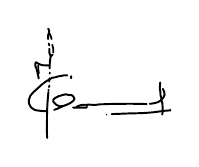
\begin{tikzpicture}[x=0.00083cm,y=-0.00083cm,line cap=round,line join=round]
\draw[line width=0.7pt] (496,250) .. controls (520,262) and (512,292) .. (507,314) .. controls (493,339) and (491,374) .. (496,410);
\draw[line width=0.65pt] (518,327) .. controls (533,350) and (540,381) .. (549,410);
\draw[line width=0.65pt] (503,478) -- (514,509);
\draw[line width=0.65pt] (559,499) .. controls (577,529) and (574,576) .. (573,620);
\draw[line width=0.7pt] (516,560) .. controls (506,603) and (517,650) .. (536,679) .. controls (549,675) and (560,665) .. (566,651);
\draw[line width=0.7pt] (533,684) .. controls (524,749) and (515,802) .. (519,863);
\draw[line width=0.65pt] (520,926) -- (519,945);
\draw[line width=0.7pt] (517,1015) -- (512,1065);
\draw[line width=0.65pt] (516,1128) -- (508,1151);
\draw[line width=0.65pt] (502,1190) -- (501,1212);
\draw[line width=0.7pt] (499,1232) .. controls (488,1344) and (483,1431) .. (479,1521) .. controls (478,1641) and (476,1761) .. (477,1845) .. controls (477,1882) and (479,1910) .. (482,1934);
\draw[line width=0.7pt] (519,815) .. controls (477,815) and (435,818) .. (400,813) .. controls (372,803) and (336,787) .. (309,768) .. controls (298,772) and (295,801) .. (299,830) .. controls (314,851) and (325,886) .. (330,923) .. controls (338,963) and (347,999) .. (351,1018);
\draw[line width=0.6pt] (343,813) .. controls (342,864) and (347,903) .. (353,942);
\draw[line width=0.7pt] (790,971) .. controls (761,959) and (736,974) .. (712,976) .. controls (671,981) and (631,988) .. (599,1002) .. controls (564,1008) and (539,1003) .. (516,1034) .. controls (460,1060) and (409,1100) .. (356,1151) .. controls (301,1200) and (252,1238) .. (220,1287) .. controls (198,1320) and (195,1366) .. (200,1405) .. controls (207,1453) and (249,1485) .. (290,1504) .. controls (344,1518) and (410,1519) .. (479,1524);
\draw[line width=0.7pt] (849,983) -- (851,1015);
\draw[line width=0.7pt] (588,1502) .. controls (647,1485) and (712,1445) .. (783,1422) .. controls (835,1402) and (884,1373) .. (902,1335) .. controls (897,1313) and (882,1288) .. (863,1277) .. controls (840,1267) and (822,1279) .. (802,1271) .. controls (781,1257) and (760,1262) .. (731,1270) .. controls (684,1281) and (633,1297) .. (602,1320) .. controls (577,1333) and (565,1353) .. (576,1380) .. controls (601,1415) and (638,1442) .. (675,1447) .. controls (711,1453) and (751,1439) .. (788,1421);
\draw[line width=0.7pt] (881,1467) -- (1090,1467) -- (1092,1424);
\draw[line width=0.7pt] (934,1453) .. controls (974,1430) and (1014,1425) .. (1072,1423) .. controls (1121,1420) and (1169,1424) .. (1226,1427) .. controls (1281,1413) and (1342,1417) .. (1408,1413) .. controls (1515,1408) and (1628,1410) .. (1742,1408) .. controls (1840,1409) and (1924,1408) .. (2014,1413);
\draw[line width=0.7pt] (2063,1409) .. controls (2101,1400) and (2141,1406) .. (2188,1384) .. controls (2215,1370) and (2230,1360) .. (2241,1345) .. controls (2260,1330) and (2282,1306) .. (2291,1272) .. controls (2293,1239) and (2280,1210) .. (2265,1179);
\draw[line width=0.7pt] (2224,1080) .. controls (2231,1107) and (2209,1131) .. (2216,1167) .. controls (2229,1204) and (2225,1254) .. (2229,1281) .. controls (2233,1307) and (2249,1320) .. (2241,1345) .. controls (2257,1381) and (2262,1423) .. (2261,1470) .. controls (2265,1511) and (2261,1550) .. (2254,1574);
\fill (1395,1576) ellipse [x radius=11,y radius=13];
\draw[line width=0.7pt] (1476,1567) .. controls (1592,1565) and (1693,1557) .. (1807,1556) .. controls (1911,1554) and (2017,1550) .. (2121,1539) .. controls (2209,1530) and (2283,1512) .. (2377,1511) -- (2375,1499);
\end{tikzpicture}}

\medskip
\hspace*{1.6em}\uline{A. GENTIL}
\end{minipage}
\end{flushright}

\margin{11}

\cotefile{148}
\scanpage{13}
\mspage{5}

qui avec l'origine $e$ forment l'ens des pts fixes de $X_S$.
(L'ens des pts fixes sous $\mathbb Z/6\mathbb Z$ \unsure{se|est} réduit
à $e$.) Les deux pts fixes sous $\mathbb Z/3\mathbb Z$, distincts de $e$, corres-\newline
pondent aux deux triangles \unsure{co-inscrits|coinscrits} de l'hexagone $S$.
(\inserted{les deux} triplets des côtés mutuelle\unsure{m\textsuperscript{t}|ment} non adjacents.)

\uline{Décompositions cellulaires}\newline
\uline{canoniques}. Décomposition en deux faces triangulaires, par trois arêtes,
un seul sommet. Les faces triangulaires correspondent aux éléments de
$(X_S)^\zeta\setminus\{e\}$ (chaque face en contient un et un seul) i.e.
aux triangles \unsure{co-inscrits|coinscrits} de l'hexagone. Les arêtes correspondent aux trois

\margin{12}

\cotefile{148}
\scanpage{14}

\noindent
\begin{minipage}[t]{.43\linewidth}
\centering\small
U N I V E R S I T E\\
DES SCIENCES ET TECHNIQUES\\
DU LANGUEDOC\\
\texttt{-{}-{}-{}-{}-{}-{}-{}-{}-{}-{}-{}-}

Service de la Scolarité\\
MA/GJ\\
Diffusion : Liste A\\
N°: 4680
\end{minipage}\hfill
\begin{minipage}[t]{.53\linewidth}
\small\vspace{2\baselineskip}
Montpellier, le 20 octobre 1983
\end{minipage}

\begin{center}
\uline{AVIS DE SOUTENANCE D'UNE THESE DE DOCTORAT DE 3ème CYCLE}

\uline{EVOLUTION ET BIOSYSTEMATIQUE}
\end{center}

\uline{Nom et prénom de la candidate} : CHAKROUN Sa\unsure{\={\i}|ï}da

\uline{Titre de la thèse} : LES VARIATIONS SAISONNIERES DES FORMATIONS SECONDAIRES (BOIS, LIBER, CAMBIUM) DU TRONC DE TROIS ESPECES MEDITERRANEENNES, LE CHENE VERT, L'OLIVIER, ET LE MICOCOULIER : UNE ETUDE HISTOPHYSIOLOGIQUE.

\uline{Date, heure et lieu de soutenance prévus} : 28 Octobre 1983 à 9h30\\
Salle de Cours n°9 - U.S.T.L.

\uline{Nom des Directeurs de thèse} : MM. Charles HEBANT et BONNET

\uline{Désignation du laboratoire où la thèse est préparée} : Laboratoire de Biologie Végétale

\uline{Résumé de la thèse} :

Cette étude concerne l'anatomie, l'histologie et l'histo-\\
chimie des tissus conducteurs secondaires d'\textit{Olea europaea}, de \textit{Quercus ilex}, et de \textit{Celtis australis}.

Le bois et le liber du Chêne et de l'Olivier ont fait l'objet d'une étude structurale approfondie.

Le fonctionnement de la zone cambiale (ainsi que la mise en place de ses dérivés, bois et liber) et l'évolution des réserves amylacées du tronc de ces trois espèces subissent des variations importantes avec le rythme saisonnier, et dans le cas de l'Olivier, avec les alternances de production.

Chez le Chêne et le Micocoulier, la totalité du bois et du liber est différenciée au printemps et en été. Chez l'Olivier, la réactivation cambiale au printemps est plus ou moins précoce selon la charge en fruits ; de plus, seuls les arbres en faible production montrent une reprise d'activité cambiale en automne, cette dernière engendre uniquement du bois.

Chez les trois espèces, la mise en place du liber est initiée plus tardivement que dans le cas du bois. Chez les deux espèces à feuilles persistantes, la zone du liber conducteur ne disparaît jamais, par contre, chez le Micocoulier, à la fin de l'automne et pendant l'hiver, tous les tubes criblés deviennent non conducteurs en accumulant de la callose.

Parallèlement à la réactivation cambiale, on note une hydro-\\
lyse de l'amidon. L'amylogénèse est plus ou moins précoce selon l'espèce observée, et dans le cas de l'Olivier, selon la charge en fruits. Une compétition entre la croissance végé-\\
tative et le développement reproductif de l'Olivier est observée.

Tout au long de l'année, les cellules compagnes et les rayons vasculaires du Chêne et de l'Olivier possèdent une forte activité phosphohydrolasique et respiratoire.

\uline{Durée approximative des recherches ayant abouti à la thèse} : 3 ans

\uline{Composition du jury proposée} :

\begin{tabular}{ll}
MM. & D'AUZAC J.\\
& BONNET A.L.\\
& KAUMAN W.\\
& NABLI M.A\\
& THALER L.\\
& VILLEMUR P.
\end{tabular}

% Closing typescript with the autograph contours in their overlapping positions.
% The signature's alphabetic reading remains undecided.
\figure{%

\begin{tikzpicture}[x=.01cm,y=-.01cm,line width=.38pt,
  every node/.style={font=\ttfamily\fontsize{9}{11}\selectfont,inner sep=0pt}]
  \node[anchor=base west] at (154,4) {P. le Secrétaire Général,};
  \node[anchor=base west] at (14,35) {l'Attachée Principale d'Administration Scolaire};
  \node[anchor=base west] at (201,66) {et Universitaire,};
  \node[anchor=base west] at (231,127) {A. GENTIL};
  % SIGNATURE_INK_BEGIN
  \draw (275,95) -- (291,91);
  \draw[line width=.6pt] (275,95) -- (279,96);
  \draw (337,35) .. controls (333,31) and (333,44) .. (335,58)
    .. controls (335,90) and (337,125) .. (341,149);
  \draw (337,35) .. controls (339,46) and (339,55) .. (337,60);
  \draw (318,73) .. controls (321,77) and (321,83) .. (319,89)
    .. controls (317,98) and (326,105) .. (338,108);
  \draw (321,77) .. controls (321,85) and (322,91) .. (324,95);
  \draw (318,73) .. controls (325,79) and (337,69) .. (355,63);
  \draw (352,71) .. controls (358,68) and (361,65) .. (364,63);
  \draw (337,101) .. controls (343,96) and (357,96) .. (362,100)
    .. controls (367,105) and (357,109) .. (347,109);
  \draw (337,104) .. controls (341,108) and (345,108) .. (348,107);
  \draw (358,106) .. controls (375,106) and (388,101) .. (412,101)
    .. controls (430,101) and (445,107) .. (456,98);
  \draw (451,78) .. controls (454,81) and (454,86) .. (455,92)
    .. controls (458,101) and (461,111) .. (460,115)
    .. controls (459,118) and (457,119) .. (456,119);
  \draw (388,109) .. controls (430,111) and (464,109) .. (506,114);
  % Editorial marker for the undecided alphabetic reading.
  \node[anchor=base west] at (520,114) {\unsure{\phantom{A}}};
  % SIGNATURE_INK_END
\end{tikzpicture}%
}

\margin{13}

\cotefile{148}
\scanpage{15}
\mspage{6}

diagonales de l'hexagone, ou encore aux\\
trois pts d'ordre 2 distincts de $e$.

Ici encore on peut ``doubler'' la\\
décomposition cellulaire, et en \unsure{tirer|trouve}\\
une autre avec 4 sommets, \deleted{\unsure{8|6}} \inserted{12} arêtes,\\
et 8 faces (triangulaires), qui permet\\
de mieux comprendre le passage

\noindent\begin{minipage}[t]{0.34\textwidth}
\vspace{0pt}
\figure{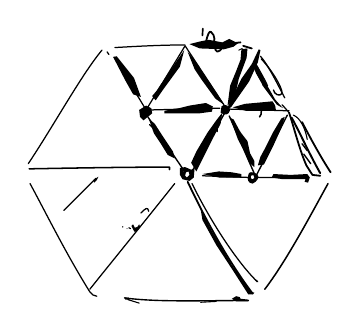
\begin{tikzpicture}[x=0.011cm,y=-0.011cm,line cap=round,line join=round]
% Interrupted outer boundary and lower rays.
\draw[line width=0.45pt] (98,33) .. controls (74,62) and (43,119) .. (13,164);
\draw[line width=0.45pt] (113,30) .. controls (147,28) and (171,27) .. (194,27);
\draw[line width=0.45pt] (15,187) .. controls (34,222) and (56,267) .. (84,312)
  .. controls (86,315) and (89,317) .. (92,317);
\draw[line width=0.45pt] (84,309) .. controls (112,274) and (152,225) .. (182,187);
\draw[line width=0.55pt] (286,309) .. controls (311,276) and (337,227) .. (359,187);
\draw[line width=0.55pt] (14,170) .. controls (69,169) and (126,168) .. (176,168)
  -- (176,171);
\draw[line width=0.65pt] (197,185) .. controls (215,223) and (241,273) .. (272,314);
\draw[line width=0.45pt] (202,187) .. controls (224,232) and (254,277) .. (276,299);
\fill (274.5,297.6) .. controls (276,297.1) and (278.8,299.1) .. (278.6,300.7)
  .. controls (277.7,302.1) and (275.1,300.6) .. (274.5,297.6);
\fill (212,217)--(225,242)--(248,281)--(270,312)--(274,313)--(272,315)
  --(267,315)--(249,287)--(230,258)--(214,229)--cycle;
% Small interior arrow, retained as its shaft and wedge.
\draw[line width=0.5pt] (54,218)--(91,181);
\fill (88,183)--(94,179)--(92,183)--(89,186)--cycle;
% Curled and dark marks on the lower-left ray.
\draw[line width=0.45pt] (143,221) .. controls (148,216) and (151,213) .. (152,219);
\fill (132,236)--(134,234)--(136,238)--(139,237)--(141,234)--(142,237)
  --(139,241)--(136,243)--(134,240)--cycle;
\fill (122,237) circle (0.8) (127,239) circle (0.55);
\draw[line width=0.4pt] (129,238)--(131,239);
% Bottom edge with its actual terminal and under-edge marks.
\draw[line width=0.5pt] (124,319) .. controls (162,324) and (210,322) .. (267,322);
\draw[line width=0.4pt] (128,321)--(141,325) (212,324)--(230,323);
\fill (248,320)--(253,317)--(257,318)--(258,320)--(267,321)
  --(267,323)--(253,323)--cycle;
\fill (124,318.4)--(129,318.8)--(130,321.2)--(125,321)--cycle;
% Upper subdivision: thin carriers and heavy irregular wedges.
\draw[line width=0.45pt] (104,35)--(106,38) (112,41)--(149,102)
  (149,102)--(194,28)--(242,101);
\fill (111,41)--(115,40)--(135,65)--(143,87)--(134,84)--(125,68)--cycle;
\fill (156,86)--(161,80)--(184,46)--(193,33)--(188,52)--(169,78)--(160,91)--cycle;
\fill (197,35)--(203,42)--(224,73)--(232,85)--(239,96)
  --(229,89)--(213,67)--(205,55)--cycle;
\draw[line width=0.45pt] (155,102)--(234,100);
\fill (170,103)--(187,100)--(199,97)--(218,94)--(226,98)--(225,104)
  --(210,106)--(187,106)--(170,106)--cycle;
\draw[line width=0.5pt] (151,110)--(194,174) (202,173)--(240,105)
  (245,109)--(275,178) (276,178)--(312,108);
\fill (152,112)--(159,118)--(168,132)--(180,150)--(182,158)
  --(174,154)--(166,141)--(158,129)--cycle;
\draw[line width=0.45pt] (153,119)--(157,123);
\fill (201,163)--(207,150)--(220,128)--(230,114)--(237,105)
  --(235,118)--(226,135)--(217,153)--(207,173)--cycle;
\draw[line width=0.5pt] (229,117)--(231,122)--(231,127);
\fill (246,111)--(250,113)--(257,126)--(259,129)--(266,138)
  --(269,152)--(274,161)--(274,168)--(268,163)--(263,151)--(255,136)--cycle;
\fill (278,166)--(281,156)--(287,145)--(296,127)--(305,112)
  --(309,110)--(306,121)--(296,143)--(285,165)--cycle;
\draw[line width=0.45pt] (244,101)--(314,103);
\fill (249,99)--(263,95)--(285,93)--(295,92)--(298,97)
  --(299,103)--(287,103)--(264,103)--cycle;
\draw[line width=0.55pt] (282,103) .. controls (283,106) and (281,108) .. (280,110);
\draw[line width=0.45pt] (214,178)--(269,180) (278,180)--(335,180);
\fill (214,176)--(233,173)--(248,174)--(259,176)--(259,180)--(233,180)--cycle;
\fill (296,176)--(316,177)--(335,176)--(338,180)--(336,186)
  --(332,185)--(333,182)--(307,182)--(294,180)--cycle;
% Top band and curls, without assigning a clean arrowhead.
\fill (199,26)--(211,23)--(221,21)--(237,24)--(245,20)
  --(255,25)--(250,29)--(239,32)--(211,31)--cycle;
\draw[line width=0.6pt] (214.5,8)--(214,16);
\draw[line width=0.65pt] (218,24) .. controls (220,15) and (222,10) .. (224,12)
  .. controls (229,16) and (229,24) .. (225,27);
\draw[line width=0.65pt] (228.7,28) .. controls (228,36) and (233,38) .. (238,28);
\draw[line width=0.65pt] (249,25)--(258,24) (261,28)--(271,31);
\draw[line width=0.35pt] (256,33)--(260,31);
% Repeated upper-right strokes.
\fill (243,97)--(246,74)--(253,57)--(258,44)--(259,32)
  --(266,31)--(265,42)--(256,66)--(251,89)--cycle;
\fill (242,101)--(259,66)--(271,49)--(279,32)--(281,33)
  --(278,47)--(268,69)--(247,99)--cycle;
\fill (271,48)--(278,52)--(285,67)--(298,90)--(307,100)
  --(300,96)--(285,76)--(276,60)--cycle;
\draw[line width=0.5pt] (282,43) .. controls (293,55) and (306,75) .. (306,83)
  .. controls (303,87) and (297,84) .. (296,79);
\draw[line width=0.5pt] (275,48) .. controls (279,55) and (286,67) .. (289,74)
  .. controls (285,76) and (282,73) .. (285,70);
\draw[line width=0.45pt] (281,40) .. controls (290,50) and (301,73) .. (309,88)
  (306,96)--(314,105);
% Repeated lower-right strokes and detached outside return.
\draw[line width=0.65pt] (314,105) .. controls (320,123) and (326,148) .. (334,166)
  -- (341,177)--(350,178);
\draw[line width=0.7pt] (317,111) .. controls (327,129) and (336,150) .. (350,175);
\draw[line width=0.65pt] (329,116) .. controls (341,139) and (351,157) .. (362,174);
\draw[line width=0.4pt] (319,108) .. controls (327,111) and (333,124) .. (335,136);
\draw[line width=0.5pt] (329,141)--(335,149) (331,153)--(339,164);
% Four marked nodes; the two lower ones retain their white openings.
\fill (141,102)--(149,97)--(155,100)--(156,106)--(146,114)--(142,110)--cycle;
\fill (236,98) .. controls (239,94) and (245,97) .. (246,102)
  .. controls (245,108) and (239,109) .. (235,105)--cycle;
\fill[even odd rule] (188,169)--(194,168)--(201,171)--(205,169)
  --(204,180)--(199,184)--(191,182)--(188,177)--cycle
  (195,174)--(198,173)--(199,177)--(196,180)--(194,178)--cycle
  (191,171)--(193,171)--(193,174)--cycle;
\fill[even odd rule] (267,177) .. controls (267,173) and (272,173) .. (277,176)
  .. controls (281,179) and (277,185) .. (272,187)
  .. controls (267,187) and (265,182) .. (267,177)--cycle
  (270,178) .. controls (272,176) and (274,177) .. (274,180)
  .. controls (273,183) and (269,183) .. (270,178)--cycle;
\end{tikzpicture}}
\end{minipage}\hfill
\begin{minipage}[t]{0.64\textwidth}
\vspace{0pt}
au quotient par $\pm1$, avec\\
quatre sommets (dont un sommet\\
privilégié, correspondant à $e$),
\end{minipage}

six arêtes les reliant $2:2$ : c'est la\\
structure tétraédrale \inserted{(orientée)}, avec un sommet\\
fixé, groupe \unsure{d'automorphismes|d'automorphisme} $\mathbb Z/3\mathbb Z$\\
(\deleted{\unsure{pourtant}} $\simeq\mathbb Z/6\mathbb Z\,/\pm1$, OK !).

\margin{14}

\cotefile{148}
\scanpage{16}

\noindent
\begin{minipage}[t]{.42\linewidth}
\centering
U N I V E R S I T E\\
DES SCIENCES ET TECHNIQUES\\
DU LANGUEDOC\\
\texttt{\textasciicircum\textasciicircum\textasciicircum\textasciicircum\textasciicircum\textasciicircum\textasciicircum\textasciicircum\textasciicircum\textasciicircum\textasciicircum\textasciicircum\textasciicircum}
\end{minipage}\hfill
\begin{minipage}[t]{.54\linewidth}
\raggedleft
\vspace*{.8\baselineskip}
Montpellier, le 14 octobre 1983
\end{minipage}

\medskip
Service de la Scolarité

Diffusion : Liste A\\
MA/gs \qquad N° 4469

\begin{center}
AVIS DE SOUTENANCE D'UNE THESE DE DOCTORAT DE 3e CYCLE

`` SCIENCES AGRONOMIQUES option PHYTOTECHNIE ''

\texttt{======================================================}
\end{center}

\uline{NOM et Prénom du candidat} : LECONTE Antoine

\uline{Titre de la Thèse} : ``LA REPRODUCTION SEXUEE DE L'HEVEA BRASILIENSIS
(UNE APPROCHE HISTOLOGIQUE ET EXPERIMENTALE)''

\uline{Date, heure et lieu de soutenance prévus} : 27 octobre 1983 à 9h.30 - Salle
de cours n°9 - (Bât. administratif ) Université des Sciences et Techniques du
Languedoc.

\uline{Nom du Directeur de thèse} : MM. Charles HEBANT - BONNET

\uline{Désignation du laboratoire où la thèse est préparée} : Laboratoire de
Biologie végétale - U.S.T.L.

\noindent\hspace*{.77\linewidth}%
\begin{tikzpicture}[x=.022cm,y=-.022cm,line cap=round,line join=round,baseline={(0,24.8)}]
\draw[line width=.65pt] (0,0)--(1.2,2.5)--(2.3,4.8)--(3.9,7.4)--(4.7,10.8)--(6.4,13.5)--(8.2,14.2)--(8.1,17.6)--(9.3,20.5)--(10.4,24.8);
\node[anchor=west] at (15,15) {\unsure{}};
\end{tikzpicture}

\uline{Analyse de l'ouvrage} : L'amélioration génétique de l'Hévéa est entravée par un
très mauvais taux de réussite des pollinisations contrôlées.

L'étude histologique montre que le processus reproducteur
(gaméto-génèse, fécondation et développement embryonnaire) se déroule normalement.
Une exception est signalée : le cas du clone GT 1 dont la stérilité mâle est
décrite. La fécondation a lieu moins de 24 heures après la pollinisation.

L'étude expérimentale, menée en Côte d'Ivoire, porte sur
les modalités de la floraison et de la fructification en conditions naturelles
et artificielles. La majorité des fleurs subissent une élimination naturelle
dans un délai de 5 à 15 jours après la pollinisation. Des traitements hormonaux
(ANA, chlorure de cobalt) peuvent augmenter significativement le taux de
fructification.

Une explication physiologique de la faible fertilité
de l'Hévéa est proposée.

\uline{Durée approximative des recherches ayant abouti à la thèse} : 2 ans

\uline{Composition du jury proposé} : \begin{tabular}[t]{ll}
MM. & BONNET\\
& D'AUZAC\\
& HALLE\\
& NICOLAS D.
\end{tabular}

\begin{flushright}
P/ le Secrétaire Général,\\
l'Attachée Principale d'Adminis-\\
tration scolaire et universitaire,

\medskip
\begin{tikzpicture}[x=.020cm,y=-.020cm,line cap=round,line join=round,baseline={(0,70)}]
% Detached left fleck and its point.
\fill (10.8,70)--(12.8,70.2)--(12.7,72.1)--(15.6,76.1)--(13.1,74.5)--(10.6,74.5)--(10,72.4)--cycle;
\fill (14.8,68.1) circle[radius=.013cm];
% Upper-left upright and separate short appendages.
\draw[line width=.50pt] (30.5,23.8) .. controls (29.3,25) and (31,27) .. (30.5,30)
 .. controls (30.2,37) and (30.2,47) .. (32.8,51.4);
\draw[line width=.48pt] (34.0,32.0)--(35.1,32.7);
\draw[line width=.48pt] (36.1,33.1) .. controls (38.0,36.7) and (40.3,38.0) .. (42.1,36.6)
 .. controls (44.5,34.9) and (45.3,32.7) .. (47.4,32.7);
\draw[line width=.45pt] (34.5,38.2) .. controls (36.7,40.7) and (35.7,43.7) .. (35.1,47.7)
 .. controls (34.7,49.7) and (33.5,50.4) .. (32.4,50.6);
% Long central descending upright.
\draw[line width=.65pt] (47.5,14.5) .. controls (49,20) and (47.5,29) .. (47.8,37.0)
 .. controls (48.1,45.0) and (46.3,53.0) .. (46.8,61.0)
 .. controls (44.7,70.0) and (44.3,77.0) .. (45.1,84.8)
 .. controls (44.4,88.9) and (47.0,93.2) .. (48.1,95.4);
% Broad left return, rising across the central upright.
\draw[line width=.60pt] (75.0,39.5) .. controls (72.1,32.1) and (59.4,35.0) .. (48.0,40.4)
 .. controls (40.0,44.6) and (28.4,48.1) .. (25.8,58.1)
 .. controls (22.4,67.7) and (31.4,69.5) .. (41.8,68.7);
% Low oval, with the small gap and point at its upper edge.
\draw[line width=.55pt] (46.9,61.2) .. controls (51.7,57.6) and (55.0,55.5) .. (57.3,54.7);
\fill (61.4,54.3) circle[radius=.0104cm];
\draw[line width=.55pt] (65.1,54.3) .. controls (68.6,53.7) and (71.0,56.5) .. (69.8,59.3)
 .. controls (68.1,63.8) and (60.7,65.3) .. (53.0,64.8)
 .. controls (50.1,64.6) and (48.3,63.7) .. (46.8,62.7);
\draw[line width=.52pt] (58.0,64.5)--(72.4,64.4);
% Upper horizontal sweep and its rising right return.
\fill (74.1,61.1)--(80.4,60.6)--(77.2,63.0)--(74.2,63.8)--cycle;
\draw[line width=.57pt] (77.7,60.9) .. controls (99.2,60.2) and (122.2,59.7) .. (133.2,59.5)
 .. controls (139.4,59.3) and (143.5,56.7) .. (145.8,52.8);
% Lower left curl and the second long horizontal sweep, with its small gap.
\draw[line width=.57pt] (72.4,66.5) .. controls (63.4,67.0) and (59.2,69.0) .. (67.6,70.0)
 .. controls (71.7,70.0) and (75.1,70.3) .. (78.2,70.6);
\draw[line width=.62pt] (82.8,70.6) .. controls (116.8,71.0) and (151.0,68.7) .. (177.0,67.1);
% Detached upper-right hook.
\draw[line width=.52pt] (142.3,37.4) .. controls (140.6,35.7) and (138.7,35.2) .. (138.2,35.3)
 .. controls (137.8,39.5) and (138.4,42.5) .. (139.4,44.2);
% Short upper segment and the attached diagonal descent at the right.
\draw[line width=.38pt] (145.8,46.5) .. controls (146.6,48.3) and (146.2,51.2) .. (145.4,53.4);
\draw[line width=.60pt] (142.5,48.6) .. controls (143.6,52.3) and (144.8,55.2) .. (147.2,58.6)
 --(152.8,68.0);
\node[anchor=west] at (181,70) {\unsure{}};
\end{tikzpicture}

\medskip
\uline{A. GENTIL}
\end{flushright}

\margin{15}

\cotefile{148}
\scanpage{18}

$4$ sommets d'ordre $6$ $+\unsure{6}$ sommets d'ordre $6$ $+12$ sommets d'ordre $3$

$24$ triangles $+4$ hexagones

% D1: upper-left pencil drawing; listing-paper stripes are not drawing strokes.
\figure{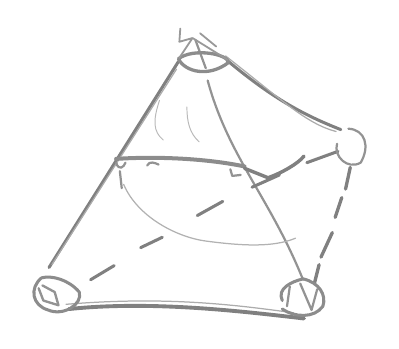
\begin{tikzpicture}[x=0.012cm,y=-0.012cm,line cap=round,line join=round]
\draw[gray,line width=1.1pt] (45,268)--(182,50) (234,49)..controls(283,90)and(316,107)..(354,122);
\draw[gray,line width=1.4pt] (66,312)..controls(153,303)and(246,314)..(315,322);
\draw[gray!65,line width=.45pt] (48,265)--(180,58) (232,44)..controls(292,91)and(318,116)..(349,124) (63,307)..controls(171,298)and(245,308)..(304,316);
\draw[gray!85,line width=.8pt] (200,27)--(211,57) (213,70)..controls(235,151)and(279,194)..(314,281);
\draw[gray,line width=1.2pt] (364,162)--(359,185) (355,194)--(348,215) (345,231)--(333,257) (331,265)--(326,285);
\draw[gray,line width=1.1pt] (89,281)--(114,266) (142,247)--(165,236) (202,213)--(229,198) (260,183)--(289,170) (318,157)--(351,145);
\draw[gray!90,line width=1.2pt] (182,47)..controls(189,61)and(214,67)..(235,51)..controls(235,42)and(198,35)..(182,47);
\draw[gray!80,line width=.65pt] (183,46)--(197,25)--(234,48) (205,20)--(222,34) (184,15)--(183,29)--(197,25);
\draw[gray!90,line width=1.1pt] (37,279)..controls(24,290)and(27,308)..(44,313)..controls(60,320)and(81,307)..(77,294)..controls(66,281)and(48,276)..(37,279);
\draw[gray!85,line width=.85pt] (38,287)--(51,294)--(55,308)--(39,303)--(34,290);
\draw[gray!90,line width=1.1pt] (292,303)..controls(286,290)and(302,283)..(314,280)..controls(331,284)and(339,297)..(335,309)..controls(326,322)and(305,321)..(292,312);
\draw[gray!85,line width=.8pt] (311,285)--(323,313)--(329,291) (300,288)--(297,309);
\draw[gray!85,line width=.8pt] (362,121)..controls(380,122)and(385,140)..(375,157)..controls(361,165)and(346,150)..(350,137);
\draw[gray!90,line width=1.45pt] (116,153)..controls(162,150)and(214,153)..(252,161);
\draw[gray!85,line width=.8pt] (116,157)..controls(119,166)and(124,162)..(126,157) (120,166)--(122,184) (149,160)..controls(151,155)and(157,157)..(161,159) (237,164)--(239,171)--(248,170);
\draw[gray,line width=1.25pt] (252,163)--(277,173)..controls(291,168)and(309,158)..(315,150);
\draw[gray!60,line width=.45pt] (124,180)..controls(139,215)and(181,236)..(211,240)..controls(249,245)and(282,247)..(306,237);
\draw[gray!55,line width=.35pt] (162,91)..controls(155,112)and(155,124)..(166,133) (191,98)..controls(191,114)and(194,126)..(204,135);
\end{tikzpicture}}

% D2: upper-right drawing, with six black interior marks and five red junctions.
\figure{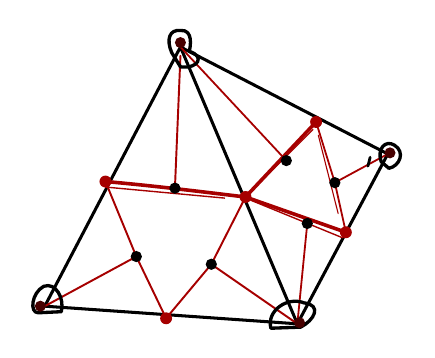
\begin{tikzpicture}[x=0.014cm,y=-0.014cm,line cap=round,line join=round]
\draw[line width=1.1pt] (28,259)--(151,24)--(339,121)--(257,275)--cycle (151,24)--(257,275);
\draw[red!65!black,line width=1.3pt] (83,146)..controls(129,150)and(176,156)..(210,160)--(301,192) (210,160)--(274,92);
\draw[red!65!black,line width=.5pt] (83,151)--(191,161) (215,163)--(298,197) (213,157)--(271,99);
\draw[red!65!black,line width=.7pt] (151,32)--(146,152) (83,146)--(111,214)--(138,270)--(179,221)--(210,160) (28,259)--(111,214) (257,275)--(179,221);
\draw[red!65!black,line width=.65pt] (151,24)--(247,127) (274,92)--(291,147)--(301,192) (339,121)--(291,147) (257,275)--(266,184);
\draw[red!65!black,line width=.4pt] (276,104)--(294,175);
\foreach \p in {(83,146),(210,160),(301,192),(138,270),(274,92)}{\fill[red!65!black] \p circle (5.4);}
\foreach \p in {(146,152),(111,214),(179,221),(247,127),(291,147),(266,184)}{\fill \p circle (5.1);}
\draw[line width=1pt] (321,132)--(323,124);
\draw[line width=1.2pt] (22,265)..controls(14,265)and(16,247)..(27,241)..controls(38,237)and(46,252)..(43,264)--cycle;
\draw[line width=1.2pt] (143,29)..controls(138,17)and(141,8)..(151,9)..controls(163,8)and(160,24)..(159,28)..controls(173,32)and(168,44)..(151,42)--(143,29);
\draw[line width=1.2pt] (233,279)..controls(229,263)and(248,250)..(263,256)..controls(280,258)and(272,272)..(260,278)--cycle;
\draw[line width=1.2pt] (333,128)..controls(329,116)and(337,108)..(345,113)..controls(355,119)and(350,132)..(340,134)--cycle;
\foreach \p in {(24,259),(151,20),(259,274),(341,120)}{\fill[red!28!black] \p circle (5);}
\end{tikzpicture}}

\margin{mieux\par cf verso\par (subdivision\par barycentrique)}

\[
\begin{aligned}
s_0&=4+6+\unsure{4}.3=22\\
s_1&=12+4.\unsure{9|8}=\unsure{48}\\
s_2&=4.7=28
\end{aligned}
\]

% D3: upper sphere, irregular small contours and actual separated point marks.
\figure{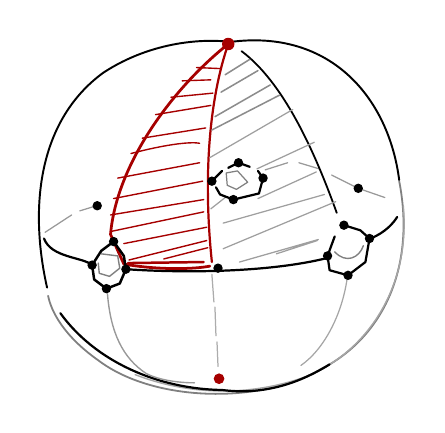
\begin{tikzpicture}[x=0.013cm,y=-0.013cm,line cap=round,line join=round]
\draw[line width=.7pt] (33,261)..controls(15,181)and(25,97)..(88,51)..controls(137,19)and(189,18)..(212,21)..controls(311,8)and(367,77)..(377,156);
\draw[gray,line width=.65pt] (377,157)..controls(393,239)and(363,309)..(300,341)..controls(241,375)and(137,373)..(83,332)..controls(49,308)and(37,284)..(34,269);
\draw[gray!70,line width=.5pt] (381,181)..controls(389,268)and(337,331)..(280,350)..controls(225,368)and(168,365)..(119,346);
\draw[line width=.8pt] (46,286)..controls(80,333)and(141,360)..(204,361)..controls(251,367)and(286,350)..(309,336);
\draw[line width=.8pt] (30,213)..controls(37,232)and(68,231)..(77,239) (110,243)..controls(169,247)and(251,246)..(307,232) (349,213)..controls(364,207)and(372,197)..(375,192);
\draw[gray!80,line width=.45pt] (31,207)--(57,190) (65,186)--(78,182) (246,146)--(268,139) (279,139)--(299,145) (311,151)--(337,164)--(363,173);
\draw[red!65!black,line width=1pt] (210,23)..controls(157,65)and(101,139)..(95,209)--(108,238)..controls(142,244)and(177,243)..(192,240);
\draw[red!65!black,line width=.8pt] (210,23)..controls(192,75)and(185,150)..(194,236);
\draw[line width=.65pt] (223,30)..controls(263,60)and(293,124)..(316,188);
\draw[gray!70,line width=.45pt] (326,253)..controls(321,287)and(304,321)..(281,337);
\draw[gray!80,line width=.5pt] (92,267)..controls(95,305)and(107,330)..(130,345)..controls(144,352)and(164,354)..(177,354);
\draw[gray!65,line width=.45pt] (194,248)--(196,275) (197,280)--(198,308) (199,314)--(200,338);
\draw[red!65!black,line width=.5pt] (179,46)--(202,47) (165,59)--(193,58) (154,75)--(195,71) (139,92)--(193,83) (126,115)--(188,105) (115,130)..controls(145,122)and(172,118)..(182,120) (102,154)--(182,139) (98,174)--(185,157) (95,190)--(186,175) (96,206)--(186,187) (108,218)--(189,202) (113,234)--(189,215) (147,233)--(190,222);
\draw[red!65!black,line width=.9pt] (112,237)--(186,236);
\draw[gray!90,line width=.55pt] (207,53)--(231,38) (203,70)--(239,49) (197,94)--(251,63) (194,107)--(260,73);
\draw[gray!75,line width=.45pt] (192,134)--(273,87) (238,145)--(294,119) (193,184)--(207,173) (239,174)--(296,148) (205,198)--(304,170) (205,223)--(315,177) (221,236)--(298,214) (257,228)--(297,215);
\draw[line width=.9pt] (98,216)--(108,230)--(110,243)--(104,257)--(91,262)--(79,253)--(77,239)--(86,225)--(98,216);
\draw[gray,line width=.5pt] (86,228)--(102,230)--(104,242)--(94,250)--(84,247)--(83,237);
\draw[line width=.8pt] (194,157)--(204,147) (210,144)--(220,139)--(231,143) (239,147)--(244,154)--(240,169)--(215,175)--(202,170)--(198,163);
\draw[gray,line width=.45pt] (208,149)--(219,147)--(229,158)--(218,165)--(209,161)--cycle;
\draw[line width=.8pt] (323,200)--(339,205)--(348,213)--(344,236)--(327,249)--(309,244)--(307,230)--(314,211);
\draw[gray,line width=.5pt] (314,226)..controls(325,238)and(338,232)..(342,220);
\foreach \p in {(98,216),(110,243),(91,262),(77,239),(194,157),(220,139),(244,154),(215,175),(323,200),(348,213),(327,249),(307,230),(82,181),(200,242),(337,164)}{\fill \p circle (4.6);}
\fill[red!65!black] (210,23) circle (6.1);
\fill[red!65!black] (201,350) circle (5.2);
\end{tikzpicture}}

% D4: central coloured tetrahedron. The lower oblique connector begins above
% the t of the following heading; its terminal return is drawn without an idealized head.
\figure{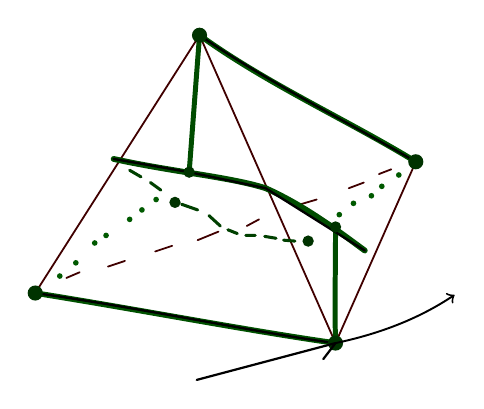
\begin{tikzpicture}[x=0.012cm,y=-0.012cm,line cap=round,line join=round]
\draw[red!25!black,line width=.65pt] (36,304)--(210,31)--(354,357)--(439,165);
\draw[green!32!black,line width=2pt] (36,304)..controls(143,321)and(262,344)..(354,357) (210,31)..controls(282,83)and(369,122)..(439,165);
\draw[line width=.85pt] (36,304)..controls(150,320)and(276,347)..(354,357) (210,31)..controls(280,79)and(365,122)..(439,165);
\draw[red!25!black,line width=.65pt] (69,288)--(83,282) (113,276)--(131,270) (163,260)--(181,254) (208,248)--(230,239) (260,233)--(273,226) (317,210)--(334,205) (368,193)--(384,187) (400,178)--(413,173);
\draw[green!30!black,line width=2.1pt] (119,162)..controls(183,176)and(242,181)..(280,193)..controls(323,212)and(363,243)..(385,259);
\draw[green!30!black,line width=1.8pt] (210,31)--(199,176) (354,234)..controls(354,278)and(353,318)..(354,357);
\draw[line width=.85pt] (119,162)--(199,176)--(280,193)--(385,259);
\draw[green!25!black,line width=1.1pt] (136,174)--(148,181) (158,187)--(169,195) (191,210)--(208,216) (220,222)--(232,233) (240,237)--(250,241) (259,243)--(269,243) (279,244)--(291,246) (299,248)--(311,249);
\foreach \p in {(62,286),(79,272),(99,251),(111,243),(136,226),(149,216),(164,205),(358,221),(373,209),(392,201),(403,191),(421,179)}{\fill[green!35!black] \p circle (3);}
\foreach \p in {(184,208),(325,249),(199,176),(354,234)}{\fill[green!20!black] \p circle (6);}
\foreach \p in {(36,304),(210,31),(354,357),(439,165)}{\fill[green!20!black] \p circle (8);}
\draw[->,line width=.7pt] (354,357)..controls(411,345)and(450,326)..(480,306);
\draw[line width=.8pt] (207,396)--(354,357)--(341,374);
\end{tikzpicture}}

\margin{ça fait $2^{\unsure{9|4}}-1=15$\par possibilités \unsure{inversion|limites}\par des faces choisies\par \unsure{en} \illegible{2} \unsure{de}\par vue !}

\uline{$4$ types de points-base}

$\bullet$ $3$ structures carrées sur $I$ (ou $J$)

$\textcolor{red!70!black}{\bullet}$ $2$ structures tétraédrales $=$ \unsure{orientation|orientations}\margin{des faces}

$\textcolor{red!30!black}{\bullet}$ $6$ structures \inserted{bi}pantaloniques\margin{opposées}\par
\hspace*{1em}(maillot ceinturé)\par
\hspace*{1em}(carrée $+$ codiagonale) $\simeq$\par
\hspace*{3em}repère de $J$)

\[
\updownarrow
\]

$\bullet$ $6$ structures pantaloniques\par
\hspace*{3em}de guingois\par
\hspace*{1em}(quart de tour)\par
(\unsure{$\simeq|=$} carré, $+$ orientation de $I$ i.e.)\par
\hspace*{4em}de $J$ $\simeq$ repère de $J$)

% F1: the raised looped glyph is preserved graphically; its alphabetic/numeric identity is open.
\margin{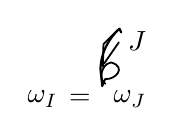
\begin{tikzpicture}[x=.75cm,y=.75cm,line cap=round,line join=round,baseline=(wI.base)]
\node[inner sep=0pt] (wI) at (0,0) {$\omega_I$};
\node[inner sep=0pt] at (.63,0) {$=$};
\node[inner sep=0pt] at (1.48,0) {$\omega_J$};
\draw[line width=.8pt] (1.01,.22)--(.98,.50)..controls(.98,.78)and(1.13,1.04)..(1.30,1.19)--(1.33,1.13);
\draw[line width=.65pt] (1.06,.26)..controls(.95,.32)and(.98,.59)..(1.16,.62)..controls(1.43,.54)and(1.23,.32)..(1.06,.34)--(1.01,.22);
\draw[line width=.65pt] (1.04,.60)--(1.29,.96) (1.02,.55)--(1.03,.93)--(1.27,1.17);
\node[inner sep=0pt] at (1.60,.99) {$J$};
\node[inner sep=0pt] at (1.86,.63) {$\unsure{\phantom{A}}$};
\end{tikzpicture}}

\diagram{\begin{tikzcd}[ampersand replacement=\&]
\operatorname{rep}(J) \arrow[d,leftrightarrow]\\
J\times\omega_J
\end{tikzcd}}

% D5: lower small sphere; the central open double-bowed contour is drawing ink.
\figure{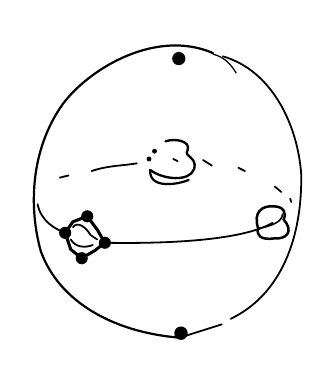
\begin{tikzpicture}[x=.014cm,y=-.014cm,line cap=round,line join=round]
\draw[line width=.8pt] (179,21)..controls(128,-1)and(68,34)..(43,67)..controls(13,109)and(12,162)..(23,201)..controls(40,247)and(89,274)..(148,279);
\draw[line width=.65pt] (188,24)..controls(233,37)and(256,87)..(259,131)..controls(260,188)and(241,240)..(195,262) (187,267)--(149,279);
\draw[line width=.45pt] (179,22)..controls(190,25)and(195,31)..(200,39);
\draw[line width=.65pt] (20,158)..controls(23,174)and(37,181)..(45,184) (81,193)..controls(138,194)and(205,191)..(233,175);
\draw[line width=.65pt] (40,134)--(48,132) (69,128)..controls(83,123)and(99,123)..(110,121) (170,118)--(178,123) (202,125)--(208,128) (235,142)--(241,147) (249,153)--(250,156);
\fill (121,117) circle (2.2); \fill (126,110) circle (2.2);
\draw[line width=.65pt] (143,117)--(147,119);
\draw[line width=.85pt] (136,101)..controls(145,98)and(159,101)..(156,109)..controls(152,115)and(165,115)..(162,126)..controls(158,138)and(134,136)..(122,127);
\draw[line width=.8pt] (122,127)..controls(121,145)and(148,140)..(157,136);
\draw[line width=1.1pt] (45,184)--(52,174)--(65,169)--(74,181)--(81,193)--(72,200)--(60,207)--(50,199)--cycle;
\draw[line width=.65pt] (52,179)..controls(56,173)and(64,179)..(68,186)--(74,190) (50,190)..controls(54,197)and(63,198)..(70,195);
\foreach \p in {(45,184),(65,169),(81,193),(60,207)}{\fill \p circle (5.5);}
\draw[line width=.9pt] (220,180)..controls(215,165)and(224,159)..(234,160)..controls(243,160)and(246,166)..(243,172)..controls(253,183)and(245,190)..(235,189)..controls(222,191)and(218,186)..(220,180);
\draw[line width=.55pt] (220,180)..controls(232,178)and(242,174)..(242,167);
\fill (148,26) circle (6); \fill (150,275) circle (6.1);
\end{tikzpicture}}

% D6: four-holed small drawing; open upper contours and unequal central strokes.
\figure{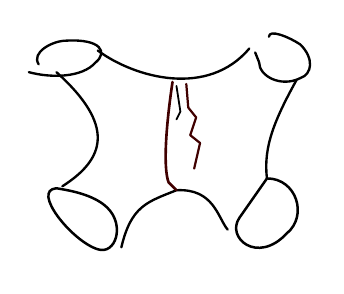
\begin{tikzpicture}[x=.025cm,y=-.025cm,line cap=round,line join=round]
\draw[line width=.85pt] (52,23)..controls(71,37)and(108,47)..(129,22) (31,34)..controls(61,61)and(56,78)..(34,92) (153,38)..controls(142,58)and(136,72)..(138,88) (64,123)..controls(69,102)and(77,100)..(92,94)..controls(111,93)and(113,108)..(118,114);
\draw[line width=.85pt] (22,30)..controls(18,24)and(29,18)..(36,18)..controls(54,17)and(57,24)..(51,29)..controls(44,37)and(28,37)..(17,34);
\draw[line width=.85pt] (139,16)..controls(139,12)and(149,16)..(155,20)..controls(162,27)and(161,35)..(155,37)..controls(145,42)and(134,36)..(134,29)--(132,24);
\draw[line width=.9pt] (31,93)..controls(18,94)and(39,120)..(52,124)..controls(61,127)and(66,112)..(57,103)..controls(50,96)and(37,94)..(31,93);
\draw[line width=.9pt] (138,88)..controls(153,88)and(159,107)..(148,116)..controls(133,132)and(117,118)..(124,108)--(138,88);
\draw[red!25!black,line width=.95pt] (90,39)..controls(87,59)and(85,82)..(88,90)--(92,94);
\draw[red!25!black,line width=.8pt] (97,40)--(98,52)--(102,57)--(99,66)--(104,70)--(101,83);
\draw[line width=.65pt] (92,41)--(94,54)--(92,58);
\end{tikzpicture}}

\margin{sur cette figure, on\par voit à la fois la \unsure{p.r.q.|proj.}\par du tétraèdre à la\par configuration-carré,\par et à la configuration\par bien pantalonique\par du guin-gois.}

% D7: lower large truncated drawing; the short corner tips and bowed trace are pencil.
\figure{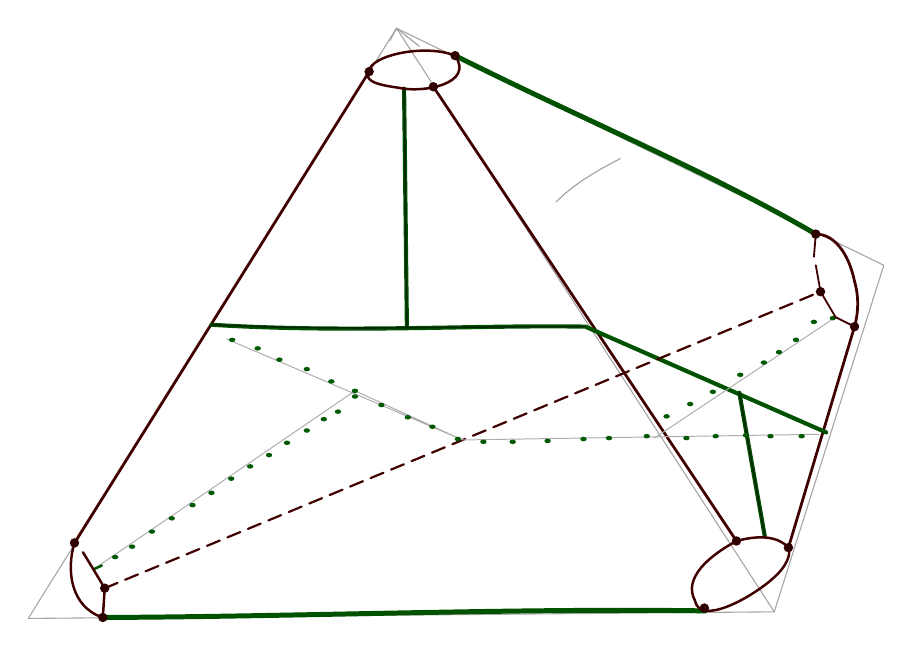
\begin{tikzpicture}[x=.012cm,y=-.012cm,line cap=round,line join=round]
\draw[gray!70,line width=.4pt] (20,642)--(410,17)--(926,268)--(810,635)--cycle (410,17)--(810,635);
\draw[gray!75,line width=.4pt] (403,30)--(410,17)--(434,36) (579,201)..controls(599,181)and(622,168)..(647,155);
\draw[red!25!black,line width=1pt] (69,562)--(381,63) (449,79)--(770,560) (825,567)--(895,333);
\draw[green!32!black,line width=1.8pt] (472,46)..controls(612,116)and(737,167)..(854,235) (99,641)..controls(313,640)and(539,631)..(737,634);
\draw[green!32!black,line width=1.5pt] (214,331)..controls(362,340)and(491,331)..(610,333)--(865,445) (418,81)--(421,334) (773,403)--(800,555);
\draw[green!15!black,line width=.55pt] (214,331)..controls(362,338)and(491,332)..(610,333) (418,81)--(421,334) (773,403)--(800,555);
\draw[red!25!black,dash pattern=on 5pt off 3pt,line width=.8pt] (101,610)--(859,296);
\draw[gray!65,line width=.35pt] (89,590)--(366,401)--(480,453)--(857,447) (230,346)--(480,453) (683,451)--(875,323);
\foreach \p in {(112,577),(130,566),(151,550),(172,536),(194,522),(214,509),(235,494),(255,481),(275,469),(294,456),(315,443),(333,431),(348,423),(366,407),(236,347),(263,356),(286,368),(315,378),(341,391),(366,401),(394,416),(422,429),(448,439),(475,452),(502,455),(533,455),(570,454),(608,452),(635,451),(675,449),(717,451),(748,449),(780,448),(806,449),(839,449),(696,428),(721,415),(745,402),(774,384),(799,371),(815,360),(833,347),(852,328),(872,324)}{\fill[green!35!black] \p ellipse (3.4 and 2.4);}
\draw[green!35!black,line width=.9pt] (89,590)--(98,586);
\draw[red!25!black,line width=.9pt] (381,63)..controls(381,46)and(440,33)..(472,46)..controls(493,76)and(438,86)..(412,80)..controls(390,77)and(375,73)..(381,63);
\draw[red!25!black,line width=.9pt] (69,562)..controls(60,591)and(65,630)..(99,641) (99,641)--(101,610)--(89,590)--(78,572);
\draw[red!25!black,line width=1pt] (854,235)..controls(874,235)and(889,256)..(895,285)..controls(902,309)and(896,329)..(895,333);
\draw[red!25!black,line width=.65pt] (854,235)--(852,259) (854,268)--(859,296)--(875,323)--(895,333);
\draw[red!25!black,line width=.9pt] (770,560)..controls(742,575)and(713,599)..(726,623)..controls(731,650)and(784,621)..(807,601)..controls(824,587)and(828,573)..(825,567)..controls(813,554)and(792,554)..(770,560);
\foreach \p in {(69,562),(101,610),(99,641),(381,63),(472,46),(449,79),(770,560),(825,567),(736,631),(854,235),(859,296),(895,333)}{\fill[red!18!black] \p circle (5);}
\end{tikzpicture}}

$4$ \uline{types de chemins élémentaires}$^{*}$

a) ``quart de twist'' $(2\times3\times4\unsure{)}$\par
\hspace*{2em}(contour d'un trou)

b) ``sixième de tour'' $(2\times2\times3)$\par
\hspace*{2em}(sur équateur)

c) pôle vers trou $(2\times2\times3)$\par
\hspace*{2em}et inv.

d) pôle vers équateur\par
\hspace*{2em}et inv. $(2\times2\times3)$

$2$ types composés supplém.

e) trou vers trou $(2\times3)$\par
\hspace*{2em}ou ``tiers de tour''

f) demi twist $(2\times2\times3)$

[et bien sûr, g) twist complet $2\times2\times3)$]

\uline{relations} ...

% D8: bottom sphere; rear equatorial arrow ends before the rear-left point.
\figure{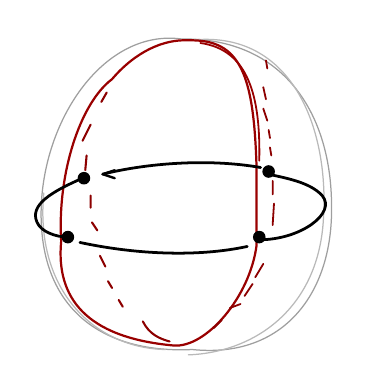
\begin{tikzpicture}[x=.017cm,y=-.017cm,line cap=round,line join=round]
\draw[gray!75,line width=.45pt] (129,18)..controls(70,10)and(23,81)..(24,151)..controls(25,222)and(72,253)..(137,250)..controls(205,257)and(242,208)..(241,143)..controls(241,76)and(207,17)..(129,18);
\draw[gray!55,line width=.45pt] (135,19)..controls(211,10)and(239,84)..(235,151)..controls(232,218)and(185,252)..(134,254) (26,133)..controls(19,207)and(65,249)..(117,250);
\draw[red!60!black,line width=.8pt] (134,19)..controls(173,18)and(183,44)..(185,115)--(185,172)..controls(180,211)and(147,249)..(123,247)..controls(57,241)and(35,211)..(39,169)..controls(36,119)and(53,66)..(77,48)..controls(94,28)and(115,18)..(134,19);
\draw[red!60!black,line width=.65pt] (143,21)..controls(179,26)and(188,61)..(187,109);
\draw[red!55!black,line width=.75pt] (73,58)--(69,65) (61,82)--(55,94) (58,105)--(57,116) (61,135)--(61,144) (62,155)--(66,161) (68,180)--(72,188) (74,199)--(77,204) (82,213)--(85,218) (100,229)..controls(105,239)and(113,242)..(120,244);
\draw[red!55!black,line width=.65pt] (192,34)--(193,40) (190,54)--(192,63) (190,70)--(193,79) (194,86)--(195,92) (195,99)--(196,105) (197,124)--(197,134) (198,141)--(197,157) (190,186)--(184,196) (182,201)--(176,210) (173,216)--(165,219) (159,228)--(153,234);
\draw[line width=1pt] (55,122)..controls(32,132)and(15,142)..(21,155)..controls(24,162)and(35,166)..(44,166) (53,170)..controls(95,179)and(141,181)..(178,173) (187,168)..controls(218,168)and(245,148)..(234,135)..controls(225,125)and(207,122)..(194,119);
\draw[line width=1pt] (188,114)..controls(148,107)and(102,111)..(70,119);
\draw[line width=.85pt] (79,116)--(70,119)--(79,122);
\foreach \p in {(56,122),(194,117),(44,166),(187,166)}{\fill \p circle (4.7);}
\end{tikzpicture}}

\margin{17}

\margin{$*$ avec les deux sens de parcours, cela\par fait \uline{huit} types de déformations,\par à visualiser a) du pt de vue conforme\par b) du pt de vue combinatoire (ici\par encore, deux pts de vue possibles)}

\cotefile{148}
\scanpage{19}

\begin{flushright}
\begin{tikzpicture}[x=.45cm,y=.45cm]
\foreach \x in {0,1,2,3} {\fill (\x,0) circle[radius=.013cm];\fill (\x+.13,0) circle[radius=.013cm];\fill (\x+.065,-.12) circle[radius=.014cm];}
\end{tikzpicture}
\end{flushright}

\noindent\hfill\begin{minipage}[t]{.50\textwidth}\vspace{0pt}
\figure{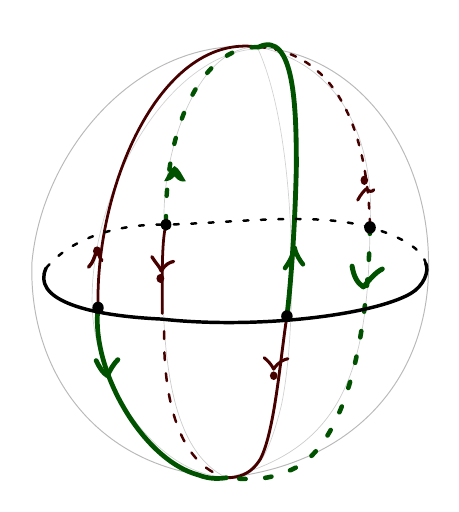
\begin{tikzpicture}[x=.012cm,y=-.012cm,line cap=round,line join=round]
\draw[gray!55,line width=.35pt] (245,19)..controls(118,7)and(16,128)..(5,247)..controls(1,364)and(75,468)..(211,475);
\draw[gray!55,line width=.35pt] (245,19)..controls(353,27)and(424,130)..(425,246)..controls(427,368)and(348,460)..(211,475);
\draw[gray!35,line width=.25pt] (240,21)..controls(143,30)and(63,180)..(69,299)..controls(74,384)and(145,476)..(213,474);
\draw[gray!35,line width=.25pt] (244,20)..controls(286,111)and(287,315)..(269,399)..controls(252,467)and(236,476)..(211,475);
\draw[gray!40,line width=.25pt] (246,19)..controls(178,15)and(142,134)..(145,207)..controls(139,351)and(153,447)..(211,475);
\draw[gray!40,line width=.25pt] (246,19)..controls(357,45)and(367,158)..(363,210)..controls(361,351)and(340,444)..(211,475);
\draw[red!28!black,line width=1pt] (245,19)..controls(142,3)and(72,165)..(75,295);
\draw[red!28!black,line width=.9pt,dash pattern=on 2.1pt off 3.7pt] (246,19)..controls(334,26)and(361,120)..(363,210);
\draw[red!28!black,line width=1pt] (147,207)..controls(142,224)and(143,271)..(143,301);
\draw[red!28!black,line width=.9pt,dash pattern=on 2.8pt off 4.8pt] (145,320)..controls(144,390)and(160,461)..(211,475);
\draw[red!28!black,line width=1.05pt] (275,304)..controls(268,349)and(262,426)..(247,455)..controls(236,473)and(222,475)..(211,475);
\draw[green!32!black,line width=1.75pt] (245,19)..controls(283,1)and(285,84)..(285,145)..controls(284,197)and(280,263)..(275,304);
\draw[green!32!black,line width=1.6pt,dash pattern=on 2.2pt off 7.3pt] (244,19)..controls(185,18)and(145,104)..(147,207);
\draw[green!32!black,line width=1.7pt] (75,295)..controls(67,360)and(122,456)..(181,472)..controls(194,477)and(204,476)..(211,475);
\draw[green!32!black,line width=1.65pt,dash pattern=on 2.3pt off 7.1pt] (363,210)..controls(361,320)and(340,433)..(285,464)..controls(256,479)and(235,477)..(211,475);
% The eight colored heads are traced as exposed strokes, without ideal arrow tips.
\draw[red!28!black,line width=1.25pt] (65,252)..controls(70,247)and(71,241)..(74,234)..controls(76,238)and(77,243)..(79,245);
\fill[red!28!black] (74,235) ellipse[x radius=.052cm,y radius=.06cm];
\draw[red!28!black,line width=1.1pt] (350,181)..controls(353,175)and(357,171)..(359,169)..controls(362,172)and(365,173)..(367,170);
\fill[red!28!black] (357,160) ellipse[x radius=.048cm,y radius=.06cm];
\node[anchor=west,inner sep=0pt] at (371,171) {\unsure{}};
\draw[red!28!black,line width=1.2pt] (132,241)..controls(137,249)and(140,251)..(142,256)..controls(147,248)and(151,247)..(155,246);
\fill[red!28!black] (141,264) ellipse[x radius=.05cm,y radius=.057cm];
\draw[red!28!black,line width=1.1pt] (251,348)..controls(256,352)and(259,356)..(261,360)..controls(266,352)and(272,350)..(276,349);
\fill[red!28!black] (261,367) ellipse[x radius=.048cm,y radius=.055cm];
\fill[green!32!black] (156,145)..controls(151,148)and(149,154)..(145,161)..controls(151,161)and(153,159)..(156,156)..controls(160,161)and(164,162)..(168,161)..controls(164,155)and(161,147)..(156,145)--cycle;
\draw[green!32!black,line width=1.65pt] (273,253)..controls(278,246)and(282,239)..(283,231)..controls(285,240)and(289,245)..(292,249);
\draw[green!32!black,line width=1.75pt] (73,351)..controls(77,359)and(80,364)..(85,367)..controls(88,360)and(92,354)..(96,350);
\draw[green!32!black,line width=1.8pt] (344,251)..controls(346,263)and(350,269)..(356,273)..controls(362,266)and(368,258)..(376,254);
\draw[black,line width=.9pt,dash pattern=on 1.8pt off 4.5pt] (20,253)..controls(52,215)and(109,206)..(147,207)..controls(222,205)and(305,193)..(363,210)..controls(398,220)and(419,234)..(422,248);
\draw[black,line width=1.25pt] (20,253)..controls(5,285)and(58,303)..(142,307)..controls(242,318)and(366,303)..(406,280)..controls(420,272)and(426,256)..(422,248);
\fill[black] (75,295) ellipse[x radius=.072cm,y radius=.077cm];
\fill[black] (275,304) ellipse[x radius=.073cm,y radius=.076cm];
\fill[black] (147,207) ellipse[x radius=.068cm,y radius=.076cm];
\fill[black] (363,210) ellipse[x radius=.074cm,y radius=.08cm];
\end{tikzpicture}}
\end{minipage}\hfill
\begin{minipage}[t]{.34\textwidth}\vspace{0pt}
passage\\
du carré\\
aux deux\\
tétraèdres
\par\medskip
Pour avoir\\
le passage aux\\
aux structures\\
pantaloniques,\\
il faut introduire\\
la \deleted{\unsure{double}}\unsure{sub}division\\
barycentrique complète\\
de la carte carrée.
\end{minipage}

\par\medskip\noindent
dans les deux cas \inserted{``spéciaux''} non digons\\
(carré, tétraèdre) les positions\\
adjacentes sont toutes ``contenues\\
dans la subdivision barycentrique

\begin{flushright}
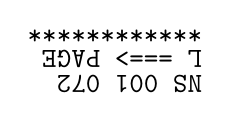
\begin{tikzpicture}
\node[rotate=180,inner sep=0pt] {\shortstack[l]{\texttt{NS 001 072}\\\texttt{L ===> PAGE}\\\texttt{************}}};
\end{tikzpicture}
\end{flushright}

\noindent\begin{minipage}[t]{.43\textwidth}\vspace{0pt}
\figure{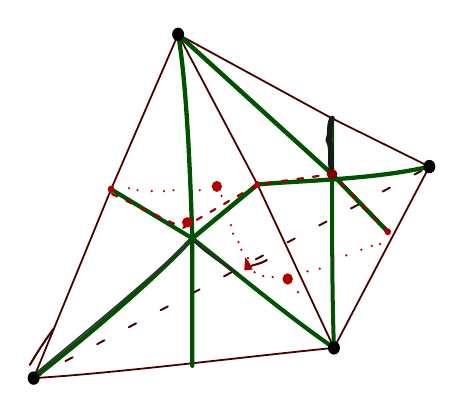
\begin{tikzpicture}[x=.012cm,y=-.012cm,line cap=round,line join=round]
\coordinate (A) at (22,383); \coordinate (B) at (175,19);
\coordinate (C) at (340,351); \coordinate (D) at (441,159);
\coordinate (O) at (190,235); \coordinate (Q) at (259,178);
\coordinate (P) at (338,167); \coordinate (J) at (338,108);
\draw[red!28!black,line width=.65pt] (A)--(104,183)--(B)--(Q)--(C)--(D)--(J)--(B);
\draw[red!28!black,line width=.65pt] (A)..controls(107,378)and(249,360)..(C);
\draw[red!28!black,line width=.7pt,dash pattern=on 3pt off 10pt] (A)--(D);
\draw[red!28!black,line width=.75pt] (18,369)..controls(25,357)and(34,343)..(43,331);
\draw[green!32!black,line width=1.55pt] (B)..controls(184,70)and(188,170)..(O)--(190,370);
\draw[green!32!black,line width=1.65pt] (A)..controls(77,340)and(147,281)..(O)--(Q);
\draw[green!32!black,line width=1.5pt] (104,183)--(O)..controls(236,271)and(293,319)..(C);
\draw[green!32!black,line width=1.6pt] (B)--(P)--(397,228);
\draw[green!32!black,line width=1.55pt] (Q)..controls(299,174)and(382,173)..(D);
\draw[green!32!black,line width=1.45pt] (J)--(P)..controls(338,228)and(338,297)..(C);
\draw[black!90,line width=2pt] (338,108)..controls(334,117)and(337,124)..(334,131)..controls(339,139)and(335,153)..(338,167);
\draw[black!80,line width=.65pt] (23,379)..controls(67,342)and(138,285)..(188,237);
\draw[black!85,line width=.65pt] (191,237)..controls(201,248)and(222,262)..(238,272);
% Red dots and broken strokes retain the unevenly drawn route.
\foreach \p in {(123,182),(132,184),(147,185),(160,185),(170,184),(198,184)} {\fill[red!70!black] \p circle[radius=.015cm];}
\draw[red!60!black,line width=.8pt,dash pattern=on 2.1pt off 3.6pt] (105,188)--(180,224)--(259,178)--(338,167)--(397,228);
\foreach \p in {(221,190),(231,221),(233,230),(239,239),(242,247),(249,256),(256,271),(265,275),(275,276),(302,292),(312,270),(325,267),(339,258),(353,253),(369,247),(380,243),(389,241)} {\fill[red!70!black] \p circle[radius=.016cm];}
\fill[red!70!black] (104,183) ellipse[x radius=.043cm,y radius=.047cm];
\fill[red!70!black] (216,180) ellipse[x radius=.065cm,y radius=.07cm];
\fill[red!70!black] (185,218) ellipse[x radius=.071cm,y radius=.065cm];
\fill[red!70!black] (259,178) ellipse[x radius=.04cm,y radius=.044cm];
\fill[red!50!black] (338,167) ellipse[x radius=.069cm,y radius=.063cm];
\fill[red!65!black] (397,228) ellipse[x radius=.042cm,y radius=.044cm];
\fill[red!70!black] (291,278) ellipse[x radius=.066cm,y radius=.072cm];
\draw[red!35!black,line width=.75pt] (269,258)..controls(263,262)and(254,263)..(247,266);
\fill[red!65!black] (246,255)--(250,260)--(254,268)--(245,269)--(246,255);
\foreach \p in {A,B,C,D} {\fill[black] (\p) ellipse[x radius=.076cm,y radius=.085cm];}
\end{tikzpicture}}
\end{minipage}\hfill
\begin{minipage}[t]{.54\textwidth}\vspace{.55cm}
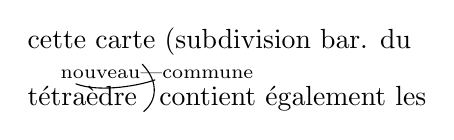
\begin{tikzpicture}[baseline=(tetra.base),line cap=round,line join=round]
\node[anchor=base west,inner sep=0pt] at (0,.72) {cette carte (subdivision bar. du};
\node[anchor=base west,inner sep=0pt] (tetra) at (0,0) {tétraèdre};
\node[anchor=base west,inner sep=0pt] at ([xshift=.27cm]tetra.base east) {contient également les};
\node[anchor=base west,inner sep=0pt,font=\scriptsize] at ([xshift=.42cm,yshift=.34cm]tetra.base west) {\inserted{\unsure{nouveau|commune}}};
\draw[line width=.4pt] ([xshift=.06cm,yshift=.52cm]tetra.base east)..controls([xshift=.28cm,yshift=.29cm]tetra.base east)and([xshift=.24cm,yshift=.05cm]tetra.base east)..([xshift=.08cm,yshift=-.08cm]tetra.base east);
\draw[line width=.4pt] ([xshift=.62cm,yshift=.27cm]tetra.base west)..controls([xshift=.94cm,yshift=.15cm]tetra.base west)and([xshift=.06cm,yshift=.26cm]tetra.base east)..([xshift=.22cm,yshift=.32cm]tetra.base east);
\end{tikzpicture}
\par\noindent
subdivisions barycentriques\\
des trois \unsure{coins|cas|cartes} ``carrés'' \unsure{associés|associées},\\
(dont l'une est marquée en\\
pointillés rouges)
\end{minipage}

\figure{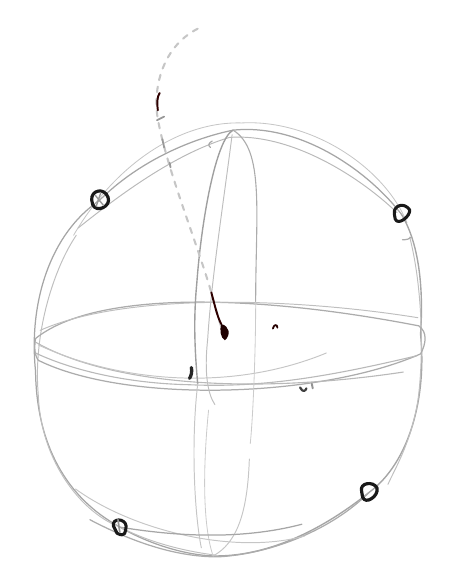
\begin{tikzpicture}[x=.0115cm,y=-.0115cm,line cap=round,line join=round]
% Pencil contours are traced separately, including their gaps and repeated passes.
\draw[gray!70,line width=.45pt] (87,198)..controls(132,153)and(191,129)..(235,120)..controls(311,112)and(386,167)..(421,213);
\draw[gray!45,line width=.3pt] (59,236)..controls(104,159)and(175,110)..(245,112)..controls(322,108)and(402,161)..(427,222);
\draw[gray!55,line width=.35pt] (64,228)..controls(119,184)and(175,145)..(231,128)..controls(297,123)and(372,169)..(416,211);
\draw[gray!70,line width=.45pt] (87,198)..controls(34,234)and(9,309)..(17,386)..controls(18,467)and(51,526)..(110,558)..controls(142,577)and(183,589)..(213,590);
\draw[gray!50,line width=.35pt] (62,236)..controls(38,271)and(14,343)..(20,412)..controls(23,489)and(71,544)..(110,558)..controls(148,578)and(191,586)..(215,589);
\draw[gray!70,line width=.5pt] (421,213)..controls(442,248)and(445,300)..(442,345)..controls(449,414)and(430,487)..(385,520)..controls(329,565)and(269,591)..(213,590);
\draw[gray!50,line width=.35pt] (430,238)..controls(444,292)and(446,368)..(439,419)..controls(431,466)and(414,493)..(406,511);
\draw[gray!65,line width=.45pt] (385,520)..controls(344,561)and(277,588)..(218,591)..controls(168,591)and(119,572)..(77,550);
\draw[gray!45,line width=.35pt] (61,516)..controls(126,563)and(238,589)..(314,568);
\draw[gray!65,line width=.45pt] (17,350)..controls(80,299)and(249,299)..(440,336)..controls(450,343)and(448,356)..(442,367)..controls(330,416)and(117,422)..(20,374)..controls(15,367)and(16,356)..(17,350);
\draw[gray!50,line width=.35pt] (22,341)..controls(119,298)and(309,306)..(439,327);
\draw[gray!55,line width=.4pt] (17,354)..controls(94,398)and(243,414)..(423,387);
\draw[gray!55,line width=.4pt] (17,366)..controls(66,389)and(131,400)..(187,401)..controls(274,405)and(353,389)..(438,369);
\draw[gray!45,line width=.35pt] (20,357)..controls(101,395)and(226,412)..(338,366);
\draw[gray!75,line width=.5pt] (235,120)..controls(216,130)and(200,220)..(195,289)..controls(191,331)and(193,366)..(196,400);
\draw[gray!45,line width=.35pt] (196,400)..controls(188,469)and(193,547)..(200,581);
\draw[gray!50,line width=.35pt] (234,125)..controls(224,203)and(211,286)..(207,351)..controls(203,388)and(207,411)..(215,423);
\draw[gray!40,line width=.3pt] (208,429)..controls(202,489)and(201,555)..(213,590);
\draw[gray!65,line width=.4pt] (235,120)..controls(270,141)and(260,211)..(260,309);
\draw[gray!40,line width=.3pt] (260,310)..controls(260,365)and(257,438)..(254,466);
\draw[gray!45,line width=.35pt] (253,483)..controls(251,543)and(239,576)..(213,590);
\draw[gray!70,line width=.45pt] (109,558)..controls(170,568)and(242,573)..(311,555);
% Four peripheral rings retain their uneven dark interiors.
\draw[black!90,line width=1.15pt] (79,197)..controls(78,186)and(93,183)..(97,194)..controls(101,204)and(84,212)..(80,202)--cycle;
\draw[gray!80,line width=.5pt] (83,192)--(92,203) (89,189)--(84,204);
\draw[black!90,line width=1.1pt] (413,212)..controls(412,203)and(424,199)..(430,208)..controls(431,215)and(417,226)..(414,218)--cycle;
\draw[black!90,line width=1.1pt] (103,557)..controls(101,548)and(116,548)..(117,557)..controls(116,563)and(117,570)..(107,565)--cycle;
\draw[gray!85,line width=.6pt] (108,550)--(110,564);
\draw[black!90,line width=1.15pt] (377,519)..controls(374,509)and(390,507)..(394,515)..controls(396,524)and(381,534)..(378,525)--cycle;
% Short exposed interior strokes are retained without added labels.
\draw[black!85,line width=1.2pt] (189,382)..controls(190,386)and(189,391)..(187,394);
\draw[black!75,line width=.8pt] (309,404)..controls(312,410)and(315,408)..(316,405);
\draw[gray!85,line width=.7pt] (322,400)--(323,405);
\draw[red!15!black,line width=.65pt] (279,339)..controls(280,334)and(284,334)..(284,338);
\draw[gray!70,line width=.4pt] (210,139)..controls(207,137)and(208,134)..(212,132);
\draw[gray!65,line width=.45pt] (422,241)..controls(427,241)and(430,240)..(432,238);
% This extended broken trace has uncertain material status; no role is assigned.
\draw[gray!45,line width=.75pt,dash pattern=on 2pt off 2.4pt] (196,8)..controls(155,29)and(145,78)..(153,113)..controls(164,168)and(194,241)..(211,299)..controls(217,322)and(222,338)..(226,349);
\draw[red!18!black,line width=.7pt] (154,79)..controls(151,83)and(151,91)..(152,98);
\draw[gray!80,line width=.65pt] (151,109)--(159,105) (157,130)--(159,139) (165,156)--(166,161);
\draw[red!18!black,line width=.7pt] (211,299)..controls(215,314)and(218,327)..(222,334);
\fill[red!12!black] (222,334)..controls(231,336)and(233,346)..(226,352)..controls(221,349)and(220,340)..(222,334)--cycle;
\node[anchor=east,inner sep=0pt] at (147,49) {\unsure{}};
\end{tikzpicture}}

\margin{18}

\begin{flushright}
\begin{tikzpicture}[x=.45cm,y=.45cm]
\foreach \x in {0,1,2,3} {\fill (\x,0) circle[radius=.014cm];\fill (\x+.13,0) circle[radius=.013cm];\fill (\x+.065,-.12) circle[radius=.014cm];}
\end{tikzpicture}
\end{flushright}

\cotefile{148}
\scanpage{20}

\figure{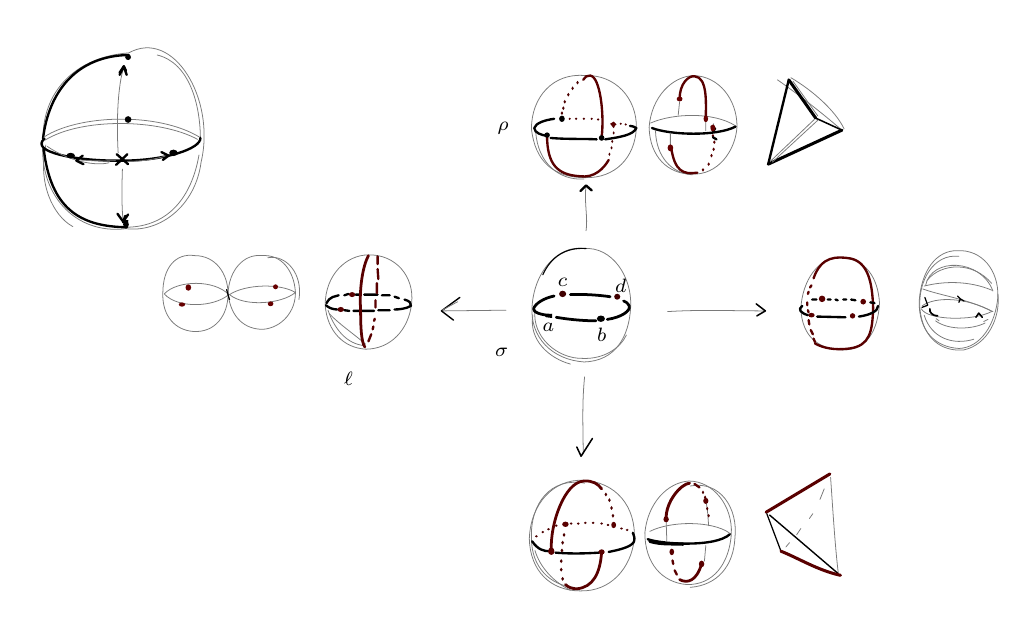
\begin{tikzpicture}[x=.009cm,y=-.009cm,line cap=round,line join=round,p/.style={draw=black!52,line width=.28pt},b/.style={draw=black,line width=.85pt},r/.style={draw=red!35!black,line width=.85pt},font=\scriptsize]
% Isolated drawing.
\draw[p] (258,88)..controls(321,53)and(381,153)..(360,242)..controls(352,304)and(302,342)..(254,336)..controls(181,345)and(130,286)..(137,210)..controls(136,145)and(180,94)..(258,88);
\draw[p] (141,218)..controls(129,271)and(151,318)..(179,333);
\draw[p] (359,210)..controls(359,162)and(344,102)..(298,91);
\draw[b] (258,91)..controls(185,92)and(145,142)..(137,209);
\draw[b] (138,224)..controls(148,307)and(188,333)..(255,334);
\draw[p] (255,334)..controls(315,333)and(347,290)..(357,232);
\draw[p] (138,207)..controls(186,175)and(299,171)..(358,207);
\draw[p] (140,211)..controls(192,179)and(302,181)..(355,210);
\draw[b] (139,209)..controls(117,228)and(185,241)..(249,240)..controls(310,240)and(360,223)..(359,208);
\draw[p] (143,220)..controls(174,241)and(211,248)..(230,243);
\draw[p] (243,229)..controls(241,197)and(241,143)..(250,111);
\draw[b] (245,119)--(251,107)--(255,119);
\draw[b] (245,116)--(251,107)--(254,113);
\draw[p] (249,252)..controls(248,279)and(248,309)..(250,324);
\draw[b] (242,315)--(250,326)--(257,316);
\draw[b] (253,318)--(250,327)--(256,325);
\draw[p] (239,240)..controls(220,241)and(203,240)..(187,239);
\draw[b] (193,233)--(184,240)--(194,245);
\draw[p] (258,241)..controls(280,241)and(300,237)..(311,233);
\draw[b] (304,228)--(314,233)--(306,239);
\draw[b] (241,231)--(257,245) (240,246)--(256,231);
\fill (257,94) circle (4.1);
\fill (257,182) circle (4.7);
\fill (176,233) ellipse (6 and 4);
\fill (321,229) ellipse (6 and 4.5);
\fill (254,330) ellipse (4 and 6);
% Upper branch.
\node at (786,194) {$\rho$};
\draw[p] (903,339)..controls(906,322)and(900,296)..(903,276);
\draw[b] (895,283)--(903,275)--(911,282);
\draw[p] (901,120)..controls(857,116)and(826,150)..(826,195)..controls(831,241)and(857,264)..(902,264)..controls(944,265)and(972,236)..(974,194)..controls(975,152)and(944,118)..(901,120);
\draw[p] (832,199)..controls(835,244)and(865,268)..(900,266);
\draw[b] (858,181)..controls(844,183)and(832,187)..(830,194)..controls(830,201)and(841,204)..(847,205);
\draw[b] (853,208)..controls(874,210)and(902,209)..(918,210);
\draw[b] (930,210)..controls(950,207)and(970,204)..(974,194)..controls(971,192)and(967,191)..(965,191);
\foreach \x/\y in {880/181,889/181,900/181,911/181,920/182,952/188,959/189}{\fill[red!30!black] (\x,\y) circle (1.7);}
\draw[r] (848,204)..controls(848,246)and(863,260)..(894,262)..controls(915,265)and(928,251)..(935,239);
\foreach \x/\y in {936/231,939/222,940/213,942/201,942/192}{\fill[red!30!black] (\x,\y) ellipse (1.5 and 2.3);}
\draw[r] (925,207)..controls(929,175)and(923,122)..(909,120)..controls(905,119)and(901,122)..(899,126);
\foreach \x/\y in {891/130,884/138,878/147,873/157,871/166,869/173}{\fill[red!30!black] (\x,\y) ellipse (1.8 and 2.6);}
\fill (848,204) ellipse (4 and 3.8);
\fill (925,208) ellipse (4 and 4);
\fill (869,181) ellipse (4 and 4.5);
\fill[red!35!black] (942,185)--(946,189)--(941,193)--(937,188)--cycle;
\draw[p] (1055,120)..controls(1024,121)and(995,151)..(992,193)..controls(993,235)and(1019,259)..(1052,259)..controls(1089,261)and(1114,226)..(1116,192)..controls(1116,153)and(1090,121)..(1055,120);
\draw[p] (1001,198)..controls(1002,235)and(1024,258)..(1053,260);
\draw[p] (994,187)..controls(1026,173)and(1083,171)..(1114,191);
\draw[b] (996,194)..controls(1022,204)and(1087,206)..(1114,192);
\draw[p] (1035,157)--(1033,176) (1072,183)--(1072,198) (1022,201)--(1022,222);
\draw[r] (1035,153)..controls(1035,132)and(1047,120)..(1056,121)..controls(1075,122)and(1072,161)..(1072,180);
\draw[r] (1023,221)..controls(1028,255)and(1040,260)..(1060,257);
\foreach \x/\y in {1068/253,1076/245,1080/233,1083/224,1084/214,1082/205}{\fill[red!35!black] (\x,\y) ellipse (1.8 and 2.5);}
\draw[b] (1082,199)--(1085,195)--(1080,192) (1082,207)--(1087,210);
\draw[p] (1083,188)--(1082,193);
\fill[red!40!black] (1035,153) ellipse (4.1 and 3.5);
\fill[red!40!black] (1072,181) ellipse (3.2 and 4.8);
\fill[red!40!black] (1022,222) ellipse (4 and 5);
\fill[red!40!black] (1082,194) ellipse (3.5 and 4.8);
\draw[p] (1173,126)..controls(1199,144)and(1235,172)..(1264,197);
\draw[p] (1192,123)..controls(1224,142)and(1255,170)..(1267,195);
\draw[b] (1189,126)--(1160,245);
\draw[b,line width=1.1pt] (1189,126)--(1227,180);
\draw[p] (1195,128)--(1230,177);
\draw[b,line width=.55pt] (1227,180)--(1264,197);
\draw[b,line width=1.1pt] (1160,245)--(1264,197);
\draw[p] (1163,241)--(1225,182);
\draw[p] (1166,242)--(1230,183);
% Left branch.
\draw[p] (351,374)..controls(324,370)and(306,391)..(306,427)..controls(305,459)and(323,479)..(349,481)..controls(380,483)and(398,458)..(398,428)..controls(398,400)and(381,374)..(351,374);
\draw[p] (446,374)..controls(420,371)and(399,395)..(398,428)..controls(402,462)and(422,478)..(447,478)..controls(474,476)and(494,452)..(493,425)..controls(491,396)and(474,372)..(446,374);
\draw[p] (454,377)..controls(480,372)and(504,400)..(498,436);
\draw[p] (308,428)..controls(327,408)and(379,408)..(399,429)..controls(378,447)and(327,449)..(308,428);
\draw[p] (400,429)..controls(423,414)and(472,413)..(493,426)..controls(474,442)and(422,447)..(400,429);
\draw[b,line width=.45pt] (396,422)--(400,436);
\fill[red!40!black] (342,419) ellipse (4 and 4.5);
\fill[red!40!black] (333,443) ellipse (4.5 and 3);
\fill[red!40!black] (465,418) circle (3.5);
\fill[red!40!black] (458,442) ellipse (4 and 3.4);
\draw[p] (596,373)..controls(565,373)and(535,401)..(535,444)..controls(538,481)and(561,504)..(592,506)..controls(627,506)and(653,479)..(657,441)..controls(661,403)and(634,372)..(596,373);
\draw[p] (539,451)..controls(548,477)and(565,499)..(591,501);
\draw[p] (541,456)..controls(555,471)and(575,484)..(592,499);
\draw[b] (537,441)..controls(542,431)and(549,432)..(554,430);
\draw[b] (562,430)--(568,428);
\draw[b] (578,429)--(585,429) (590,429)--(609,429) (615,430)--(626,430) (633,432)--(639,434);
\draw[b] (647,436)..controls(654,438)and(657,441)..(656,445)..controls(649,449)and(639,450)..(633,450);
\draw[b] (536,444)..controls(540,448)and(547,450)..(552,450);
\draw[b] (562,451)--(569,452) (575,452)--(604,452) (610,451)--(626,451);
\fill[red!35!black] (573,429) ellipse (4.5 and 3.5);
\fill[red!35!black] (557,450) ellipse (4.6 and 3.6);
\draw[r,line width=1pt] (596,374)..controls(588,389)and(583,420)..(585,451)..controls(585,475)and(586,496)..(591,503);
\draw[r] (609,375)--(609,386) (609,393)--(610,407) (608,413)--(608,427) (606,437)--(606,447);
\draw[r] (605,463)--(604,466) (603,474)--(602,478) (600,485)--(596,495);
\node at (568,548) {$\ell$};
\draw[p] (790,451)--(701,452);
\draw[b,line width=.5pt] (725,433)--(699,452)--(716,465);
\draw[p] (722,439)--(700,451);
\node at (784,511) {$\sigma$};
% Central sphere.
\draw[p] (900,364)..controls(866,359)and(831,393)..(827,444)..controls(823,490)and(856,521)..(900,524)..controls(944,523)and(964,489)..(966,446)..controls(968,404)and(940,361)..(900,364);
\draw[b,line width=.4pt] (842,401)..controls(854,375)and(875,362)..(903,364);
\draw[p] (831,452)..controls(827,488)and(862,520)..(899,519)..controls(928,520)and(951,505)..(960,486);
\draw[p] (828,458)..controls(822,493)and(851,519)..(881,527);
\draw[b,line width=1pt] (858,431)..controls(843,434)and(831,442)..(829,449)..controls(828,454)and(841,458)..(851,458);
\draw[b,line width=1pt] (861,461)..controls(884,465)and(905,466)..(917,466);
\draw[b,line width=1pt] (933,464)..controls(953,461)and(966,452)..(964,445)..controls(961,440)and(959,439)..(956,438);
\draw[b,line width=1pt] (881,429)..controls(900,428)and(924,430)..(937,432);
\fill[red!25!black] (870,428) ellipse (5 and 4.5);
\fill[red!25!black] (947,432) ellipse (4.3 and 4.2);
\fill (842,457)--(855,456)--(855,462)--(847,461)--cycle;
\fill (924,463) ellipse (5.7 and 4.5);
\node at (870,412) {$c$};
\node at (952,416) {$d$};
\node at (850,475) {$a$};
\node at (925,485) {$b$};
% Right branch.
\draw[p] (1018,453)..controls(1063,450)and(1112,452)..(1154,452);
\draw[b,line width=.55pt] (1143,442)--(1156,452)--(1144,459);
\draw[p] (1262,377)..controls(1230,376)and(1208,410)..(1206,449)..controls(1208,488)and(1230,506)..(1265,507)..controls(1300,508)and(1315,478)..(1317,441)..controls(1315,406)and(1298,378)..(1262,377);
\draw[r] (1224,406)..controls(1235,374)and(1257,375)..(1276,378)..controls(1300,383)and(1307,410)..(1308,448)..controls(1307,482)and(1303,501)..(1275,505)..controls(1253,508)and(1237,504)..(1226,498);
\draw[r] (1221,416)--(1219,419) (1217,425)--(1216,428) (1215,440)--(1215,444) (1216,451)--(1217,454) (1217,465)--(1218,471) (1220,479)--(1223,485) (1224,491)--(1226,496);
\draw[b] (1208,445)..controls(1201,450)and(1206,455)..(1216,458);
\draw[b] (1229,460)--(1269,461);
\draw[b] (1288,460)..controls(1302,458)and(1315,453)..(1315,445);
\draw[b] (1222,436)--(1228,436) (1244,436)--(1248,436) (1255,436)--(1258,437) (1266,436)--(1270,436) (1277,436)--(1283,437) (1304,440)--(1310,441);
\fill[red!35!black] (1236,435) circle (4.6);
\fill[red!35!black] (1294,439) circle (4);
\fill[red!35!black] (1221,458) ellipse (4.5 and 3.2);
\fill[red!35!black] (1279,459) circle (3.8);
\draw[p] (1426,367)..controls(1397,367)and(1376,395)..(1373,438)..controls(1372,481)and(1396,503)..(1429,505)..controls(1460,504)and(1481,470)..(1484,432)..controls(1485,395)and(1462,365)..(1426,367);
\draw[p] (1429,375)..controls(1393,371)and(1371,410)..(1374,449)..controls(1378,491)and(1405,510)..(1436,507)..controls(1469,500)and(1488,462)..(1484,428);
\draw[p] (1382,416)..controls(1390,376)and(1460,378)..(1477,424);
\draw[p] (1384,409)..controls(1404,384)and(1449,382)..(1475,413);
\draw[p] (1380,417)..controls(1407,410)and(1443,409)..(1476,423);
\draw[p] (1378,421)..controls(1402,430)and(1441,435)..(1477,453);
\draw[p] (1377,445)..controls(1396,431)and(1441,433)..(1476,453);
\draw[p] (1376,449)..controls(1384,465)and(1448,467)..(1475,453);
\draw[p] (1396,466)..controls(1415,480)and(1449,478)..(1466,469);
\draw[p] (1380,458)..controls(1390,490)and(1420,501)..(1450,492);
\draw[b,line width=.45pt] (1381,433)--(1385,444)--(1377,447);
\draw[b,line width=.45pt] (1427,431)--(1431,435)--(1429,440) (1431,435)--(1436,438);
\draw[b,line width=.6pt] (1388,449)..controls(1387,454)and(1392,459)..(1399,459);
\draw[b,line width=.55pt] (1453,461)--(1457,455)--(1462,461);
\draw[p] (1397,463)--(1401,466) (1464,467)--(1470,464);
% Lower branch.
\draw[p] (901,545)..controls(897,583)and(899,620)..(899,654);
\draw[b,line width=.55pt] (890,644)--(896,657)--(912,632);
\draw[p] (899,691)..controls(857,689)and(825,724)..(823,773)..controls(824,819)and(853,847)..(895,847)..controls(938,848)and(966,815)..(971,775)..controls(974,728)and(945,693)..(899,691);
\draw[p] (901,695)..controls(853,686)and(824,724)..(826,773)..controls(826,813)and(852,839)..(886,842);
\draw[p] (831,790)..controls(838,814)and(858,835)..(881,846);
\draw[b] (827,777)..controls(835,789)and(844,791)..(851,791);
\draw[b] (860,793)..controls(883,795)and(907,794)..(921,793);
\draw[b] (935,792)..controls(956,788)and(970,783)..(971,776)..controls(972,771)and(970,768)..(969,765);
\foreach \x/\y in {833/770,842/764,850/760,861/755,882/752,892/752,902/751,913/751,925/752,934/754,953/759,961/761}{\fill[red!30!black] (\x,\y) ellipse (2 and 1.7);}
\draw[r,line width=1pt] (854,791)..controls(852,752)and(873,693)..(900,692)..controls(912,691)and(920,696)..(925,703);
\foreach \x/\y in {931/711,936/719,939/730,941/741}{\fill[red!30!black] (\x,\y) ellipse (1.9 and 2.8);}
\draw[r,line width=1pt] (925,792)..controls(923,822)and(913,842)..(890,844)..controls(883,844)and(878,842)..(874,838);
\foreach \x/\y in {870/830,868/817,868/805,869/790,870/779,872/768}{\fill[red!30!black] (\x,\y) ellipse (2 and 2.8);}
\fill[red!35!black] (854,791) ellipse (4.5 and 5.3);
\fill[red!35!black] (925,792) ellipse (4.3 and 3.7);
\fill[red!35!black] (874,753) ellipse (4.6 and 3.8);
\fill[red!35!black] (942,754) ellipse (3.4 and 4.5);
\draw[p] (1048,692)..controls(1018,694)and(990,723)..(986,765)..controls(986,808)and(1010,835)..(1045,838)..controls(1083,839)and(1105,808)..(1108,767)..controls(1110,726)and(1082,692)..(1048,692);
\draw[p] (1050,699)..controls(1092,691)and(1118,730)..(1113,773)..controls(1111,811)and(1089,839)..(1050,842);
\draw[p] (993,763)..controls(1023,748)and(1080,748)..(1105,765);
\draw[b] (990,774)..controls(1009,781)and(1086,786)..(1106,767);
\draw[b,line width=1.2pt] (993,777)..controls(1010,782)and(1027,780)..(1040,781);
\draw[p] (1016,748)--(1017,777) (1072,720)..controls(1075,734)and(1075,745)..(1076,755) (1072,783)--(1070,805);
\draw[r,line width=1.05pt] (1016,746)..controls(1015,721)and(1037,696)..(1049,695);
\draw[r] (1056,696)--(1063,701);
\foreach \x/\y in {1068/708,1071/715,1074/731,1076/741}{\fill[red!30!black] (\x,\y) ellipse (1.7 and 2.6);}
\draw[r,line width=1pt] (1066,809)..controls(1059,833)and(1046,837)..(1035,831);
\draw[r] (1031,824)--(1028,818) (1026,809)--(1025,804);
\fill[red!35!black] (1016,746) ellipse (3.8 and 4.2);
\fill[red!35!black] (1072,720) ellipse (3.7 and 4.3);
\fill[red!35!black] (1024,792) ellipse (3.3 and 4.6);
\fill[red!35!black] (1066,809) ellipse (3.8 and 4.7);
\draw[r,line width=1.1pt] (1157,736)--(1247,682);
\draw[p] (1248,687)..controls(1251,729)and(1254,782)..(1259,823);
\draw[b,line width=.45pt] (1158,738)--(1178,791);
\draw[b,line width=.5pt] (1162,740)--(1258,822);
\draw[r,line width=1.1pt] (1178,791)..controls(1203,801)and(1230,818)..(1262,825);
\draw[p] (1185,785)--(1190,779) (1200,768)--(1206,759) (1218,745)--(1223,738) (1233,718)--(1239,703);
\end{tikzpicture}}

% FORMULAS
\[
\begin{aligned}
I&\unsure{=|\simeq}\unsure{S_Q|I_Q}=\coprod_{d\in D_Q}d\\
A_Q&=\prod_{d\in D_Q}d\\
C_Q&=\bigwedge_{d\in D_Q}d=\perp\\
\omega_Q&=C_Q\wedge D_Q\\
\omega_I&\simeq\omega_J\simeq C_Q\simeq J\setminus\{Q\}
\end{aligned}
\]

% PARTITIONS
\figure{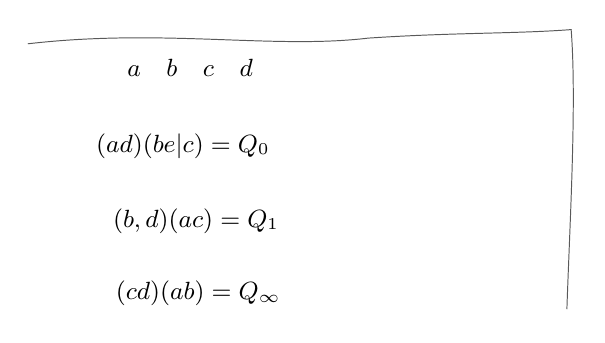
\begin{tikzpicture}[x=.018cm,y=-.018cm,line cap=round,line join=round,font=\small]
\draw[black!65,line width=.35pt] (80,997)..controls(175,986)and(253,1001)..(320,993)..controls(380,989)and(424,990)..(463,987);
\draw[black!65,line width=.35pt] (463,987)..controls(467,1038)and(462,1124)..(460,1184);
\node[anchor=west] at (143,1014) {$a\quad b\quad c\quad d$};
\node[anchor=west] at (121,1069) {$(ad)(b\unsure{e|c})=Q_0$};
\node[anchor=west] at (133,1122) {$(b,d)(ac)=Q_1$};
\node[anchor=west] at (135,1173) {$(cd)(ab)=Q_\infty$};
\end{tikzpicture}}

% EQUIVALENCE
\figure{\begin{tikzpicture}[x=.014cm,y=-.014cm,line cap=round,line join=round,font=\small]
% Weak upper pencil annotation.
\node[anchor=west,text=black!50,scale=.85,inner sep=0pt] at (858,992) {\unsure{tétraèdre $+$ b}};
\node[anchor=west,inner sep=0pt] at (1080,982) {\unsure{\begin{tikzpicture}[x=.018cm,y=-.018cm,baseline=-.5ex,line cap=round,line join=round]
\draw[black!45,line width=.3pt] (1,18)..controls(10,13)and(11,20)..(17,19);
\draw[black!45,line width=.3pt] (20,17)..controls(25,23)and(28,27)..(31,25);
\draw[black!45,line width=.3pt] (39,8)--(34,28);
\draw[black!45,line width=.3pt] (47,17)..controls(55,13)and(59,17)..(63,16);
\draw[black!45,line width=.3pt] (53,24)--(67,22);
\end{tikzpicture}}};
\node[anchor=west,text=black!50,scale=.85,inner sep=0pt] at (1193,995) {\unsure{(carré $+$}};
% Live expression and raised word.
\node[anchor=west,inner sep=0pt] at (570,1044) {(tétraèdre $+$ diagonale)};
\node[anchor=west,inner sep=0pt] at (1059,1041) {(carré $+$ codiagonale)};
\node[anchor=south,inner sep=0pt] at (709,1024) {\inserted{orienté}};
\draw[line width=.55pt] (657,1020)..controls(680,1027)and(746,1025)..(770,1017);
\draw[line width=.55pt] (713,1025)--(716,1038);
\draw[line width=1pt] (963,1038)--(1053,1037);
\draw[line width=.9pt] (978,1023)--(961,1038)--(978,1050);
\draw[line width=.9pt] (1038,1024)--(1055,1037)--(1040,1051);
% First faint line below the left term, with its intersecting leading strokes.
\node[anchor=north west,inner sep=0pt] at (631,1063) {\unsure{
\begin{tikzpicture}[x=.014cm,y=-.014cm,baseline=-.5ex,line cap=round,line join=round]
\draw[black!50,line width=.32pt] (17,3)..controls(18,11)and(21,20)..(20,29);
\draw[black!50,line width=.32pt] (1,27)--(39,22);
\draw[black!50,line width=.32pt] (7,32)..controls(19,24)and(27,12)..(34,3);
\draw[black!50,line width=.32pt] (18,20)--(43,31);
\draw[black!50,line width=.32pt] (57,10)..controls(52,22)and(50,34)..(57,34)..controls(64,32)and(66,24)..(67,19)..controls(65,35)and(77,33)..(79,18);
\draw[black!50,line width=.32pt] (82,32)--(98,33) (89,33)--(90,46) (83,46)--(99,45);
\draw[black!50,line width=.32pt] (113,18)--(132,35) (115,36)--(131,18);
\draw[black!50,line width=.32pt] (156,14)..controls(158,24)and(161,30)..(169,33)..controls(158,35)and(151,33)..(146,32);
\end{tikzpicture}}};
% Further faint formula line: exact contents remain undecided.
\node[anchor=north west,inner sep=0pt] at (682,1117) {\unsure{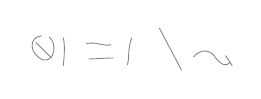
\begin{tikzpicture}[x=.014cm,y=-.014cm,baseline=-.5ex,line cap=round,line join=round]
\draw[black!48,line width=.32pt] (17,8)..controls(5,9)and(6,25)..(19,30)..controls(30,31)and(31,14)..(24,9);
\draw[black!48,line width=.32pt] (12,14)--(26,28);
\draw[black!48,line width=.32pt] (37,10)..controls(39,20)and(37,31)..(37,35);
\draw[black!48,line width=.32pt] (58,15)..controls(68,13)and(73,18)..(80,16);
\draw[black!48,line width=.32pt] (60,29)--(82,28);
\draw[black!48,line width=.32pt] (99,10)..controls(95,19)and(97,29)..(95,34);
\draw[black!48,line width=.32pt] (124,1)--(144,39);
\draw[black!48,line width=.32pt] (155,27)..controls(163,18)and(172,22)..(175,28)..controls(181,35)and(185,36)..(188,32);
\draw[black!48,line width=.32pt] (184,26)--(190,35);
\end{tikzpicture}}};
% Brace below the central span and its two formula baselines.
\draw[line width=.55pt] (884,1085)..controls(882,1096)and(895,1101)..(923,1102)..controls(955,1103)and(979,1116)..(993,1129)..controls(1005,1115)and(1022,1101)..(1050,1104)..controls(1082,1108)and(1106,1104)..(1110,1095);
\node[anchor=west,inner sep=0pt] at (941,1162) {$\omega_I\times J$};
\node[anchor=west,inner sep=0pt] at (915,1215) {$\simeq J\times\omega_I$};
\end{tikzpicture}}

% EXACT_SEQUENCE
\diagram{\begin{tikzcd}
0\arrow[r]&V(J)\arrow[r]&\unsure{\mathfrak S}_I\arrow[r]&\unsure{\mathfrak S}_J\arrow[r]&1
\end{tikzcd}}

% PENCIL_SHAPE
\figure{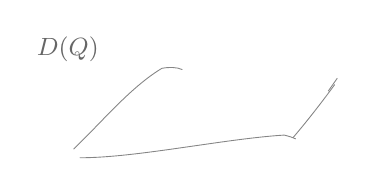
\begin{tikzpicture}[x=.016cm,y=-.016cm,line cap=round,line join=round,font=\small]
\node[anchor=west,text=black!60] at (195,1372) {$\unsure{D(Q)}$};
\draw[black!48,line width=.32pt] (232,1451)..controls(254,1430)and(277,1402)..(302,1387)..controls(307,1386)and(314,1386)..(318,1388);
\draw[black!48,line width=.32pt] (237,1458)..controls(282,1458)and(351,1443)..(399,1440)..controls(403,1441)and(406,1442)..(408,1443);
\draw[black!48,line width=.32pt] (406,1442)..controls(418,1428)and(431,1411)..(439,1400);
\draw[black!48,line width=.32pt] (434,1405)--(441,1395);
\end{tikzpicture}}

% RELATIONS
\figure{\begin{tikzpicture}[x=.015cm,y=-.015cm,line cap=round,line join=round,font=\large]
\draw[black!58,line width=.35pt] (732,1298)..controls(867,1292)and(1024,1271)..(1167,1279);
\draw[black!58,line width=.35pt] (1167,1282)..controls(1168,1372)and(1166,1483)..(1174,1549);
\draw[black!58,line width=.35pt] (711,1341)..controls(714,1423)and(713,1510)..(720,1571);
\draw[black!58,line width=.35pt] (728,1570)..controls(858,1552)and(999,1564)..(1105,1558)..controls(1109,1558)and(1111,1560)..(1113,1561);
\node[anchor=west] at (773,1418) {$\left\{\begin{aligned}\rho^3&=\sigma^2=1\\[1.1ex]\rho\sigma&=\ell\end{aligned}\right.$};
\end{tikzpicture}}

% LOWER_DIAGRAM
% Lower array: the faint overlay and hatched superscript retain their actual strokes.
% A question at either graphic locus marks the unresolved character identification.
\diagram{\begin{tikzpicture}[x=1cm,y=1cm,line cap=round,line join=round]
% Pale overwritten span beside the lower Pi; drawn before the dark label and shaft.
\draw[gray!55,line width=.35pt] (1.63,-2.61)..controls(1.49,-2.65)and(1.48,-2.87)..(1.57,-3.03);
\draw[gray!55,line width=.35pt] (1.76,-2.61)..controls(1.91,-2.55)and(2.02,-2.66)..(1.94,-2.77)--(1.78,-2.94)--(2.05,-2.96);
\draw[gray!50,line width=.35pt] (2.10,-2.96)--(2.07,-3.06);
\draw[gray!55,line width=.35pt] (2.24,-2.73)--(2.52,-2.72)--(2.25,-2.99)--(2.54,-2.99);
\draw[gray!45,line width=.3pt] (2.55,-2.73)..controls(2.69,-2.76)and(2.74,-2.90)..(2.66,-3.06);
\node[inner sep=0pt] at (2.79,-3.19) {$\unsure{\phantom{A}}$};
\node[inner sep=0pt] (u0) at (0,0) {$1$};
\node[inner sep=0pt] (u1) at (1.32,0) {$\mathcal T_{0,4}^{!}$};
\node[inner sep=0pt] (u2) at (3.79,0) {$\mathcal T_{04}$};
\node[inner sep=0pt] (u3) at (6.05,0) {$\unsure{\mathfrak S}_4$};
\node[inner sep=0pt] (u4) at (7.85,0) {$1$};
\node[inner sep=0pt] (m0) at (0,-1.51) {$1$};
\node[inner sep=0pt] (m1) at (1.32,-1.51) {$\Pi_{0,3}$};
\node[inner sep=0pt] (m2) at (3.79,-1.51) {$\mathcal T'_{04}$};
\node[inner sep=0pt] (m3) at (6.05,-1.51) {$\unsure{\mathfrak S}_3$};
\node[inner sep=0pt] (m4) at (7.85,-1.51) {$1$};
\node[inner sep=0pt] (l0) at (0,-3.00) {$1$};
\node[inner sep=0pt] (l1) at (1.32,-3.00) {$\Pi_{0,\unsure{5|3}}$};
\node[inner sep=0pt] (l2) at (3.79,-3.00) {$\mathcal T_{1,1}$};
\node[inner sep=0pt] (l3) at (6.05,-3.00) {$\widetilde{\unsure{\mathfrak S}}_3$};
\draw[->,line width=.55pt] (.22,0)--(.68,0);
\draw[->,line width=.65pt] (2.02,0)--(3.12,0);
% The upper middle arrow begins in the crossed raised cluster.
\draw[line width=.45pt] (4.25,.24)..controls(4.31,.39)and(4.42,.30)..(4.45,.20);
\draw[line width=.4pt] (4.28,.31)--(4.22,-.06) (4.35,.34)--(4.32,.02) (4.43,.29)--(4.48,-.07);
\draw[gray!75,line width=.45pt] (4.20,.16)--(4.39,.36) (4.21,.07)--(4.48,.34) (4.24,-.01)--(4.48,.23) (4.32,-.06)--(4.52,.15) (4.41,-.09)--(4.56,.07);
\node[inner sep=0pt] at (4.53,.48) {$\unsure{\phantom{A}}$};
\draw[->,line width=.65pt] (4.42,.04)--(5.40,.04);
\draw[->,line width=.65pt] (6.64,0)--(7.49,0);
\draw[->,line width=.55pt] (.22,-1.51)--(.68,-1.51);
\draw[double,double distance=.65pt,->,line width=.45pt] (2.02,-1.51)--(3.12,-1.51);
\draw[->,line width=1.1pt] (4.42,-1.51)--(5.40,-1.51);
% The middle terminal connector has a blunt upturned end, without a supplied head.
\draw[line width=.55pt] (6.63,-1.51)..controls(6.98,-1.55)and(7.24,-1.56)..(7.44,-1.53)--(7.44,-1.44);
\draw[->,line width=.55pt] (.22,-3.00)--(.68,-3.00);
\draw[double,double distance=.65pt,->,line width=.45pt] (2.29,-3.00)--(3.12,-3.00);
\draw[->,line width=.65pt] (4.43,-3.00)--(5.40,-3.00);
\draw[->,line width=.55pt] (3.79,-.47)--(3.79,-1.01);
\draw[->,line width=1pt] (6.05,-.49)--(6.05,-1.03);
\draw[->,line width=.65pt] (3.79,-2.57)--(3.79,-1.99);
\draw[->,line width=.85pt] (6.05,-2.55)--(6.05,-1.99);
\node[inner sep=0pt] at (1.32,-.72) {\rotatebox{90}{$\simeq$}};
\node[inner sep=0pt] at (1.32,-2.24) {\rotatebox{90}{$\simeq$}};
\node[inner sep=0pt] at (4.81,-.72) {cart};
\node[anchor=west,inner sep=0pt] at (6.63,-.65) {$\simeq\operatorname{Aff}(2,\mathbb Z/2\mathbb Z)$};
\node[anchor=west,inner sep=0pt] at (6.30,-2.10) {`` $\operatorname{Sl}(2,\mathbb Z/2\mathbb Z)$};
\node[anchor=west,inner sep=0pt] at (6.63,-3.00) {$\simeq\operatorname{Sl}(2,\mathbb Z/4\mathbb Z)/-$};
\node[inner sep=0pt] at (3.68,-3.78) {\rotatebox{90}{$\simeq$}};
\node[anchor=west,inner sep=0pt] at (3.98,-3.93) {$\operatorname{Sl}(2,\mathbb Z)$};
\end{tikzpicture}}

\margin{19}
